%************************************************
\chapter{Do PTAs observe a dark sector phase transition?} \label{chp:ptabbn}
%************************************************

\begin{tcolorbox}[colframe=DESYcyan, colback=DESYcyan!10]
	\textbf{This chapter is based on the following publication:}
	\begin{itemize}[leftmargin=17pt]
		\item[\cite{Bringmann:2023opz}] \bibentry{Bringmann:2023opz}
	\end{itemize}
\end{tcolorbox}
\vspace{0.5cm}

\begin{flushright}
	\slshape
	Never tell me the odds!\\ \medskip
	--- Han Solo
\end{flushright}

\section{Introduction}


In the last chapter we found that \acp{DSPT} can be the source of strong \acp{GWB}. The recent \ac{PTA} observation discussed in chapter~\ref{chp:PTAs} now leads us straight to the central question of the present chapter: \textit{Do pulsar timing arrays observe a dark sector phase transition?}

At the end of chapter~\ref{chp:PTAs} we have already identified the strongest contender for any alternative explanation of the novel signal's origin: an astrophysical \ac{GWB} emitted by inspiraling \acp{SMBHB}. In order to explain the observed signal's amplitude, however, it \graffito{Astrophysics or cosmology?} was argued that the local \ac{SMBHB} density would need to be higher by an $\mathcal{O}(10)$ factor compared to previous estimates~\cite{Casey-Clyde:2021xro, Kelley:2016gse, Kelley:2017lek}, cf.~fig.~\ref{fig:nano15astrogwcompare}. The question of whether realistic astrophysical models could give rise to a sufficiently strong \ac{GWB} hence remains the subject of an ongoing debate~\cite{Middleton:2020asl, Izquierdo-Villalba:2021prf, Curylo:2021pvf, Somalwar:2023bqv, NANOGrav:2023hfp}.

In order to match the observed \ac{GW} signal at nHz frequencies, the preferred temperature for a cosmological \ac{PT} must be at the MeV-scale~\cite{NANOGrav:2021flc, NANOGrav:2023hvm}, cf.~fig.~\ref{fig:observability}. As new physics at this 
energy scale is very strongly constrained by a large variety of direct experimental searches~\cite{Gori:2022vri}, this immediately implies that the associated new states should only couple very weakly to the \ac{SM}. In other words, such a \graffito{Stable and decaying \acp{DS}} phase transition would have to take place in a more or less secluded \ac{DS}---which could, in fact, also be directly related to the dark matter puzzle~\cite{Pospelov:2007mp,Feng:2008mu,Pospelov:2008zw}. Importantly, even if the \ac{DS} is only very weakly coupled to the \ac{SM}, a \ac{DSPT} could impact the successful predictions of \ac{BBN} and the \ac{CMB} due to the extra energy density that is present in the \ac{DS} (conventionally parameterized as an effective number of new relativistic neutrino degrees of freedom $\Delta N_\text{eff}$, see eq.~\eqref{eq:DNeff})~\cite{Planck:2018vyg,Yeh:2022heq} or through the late decay of the additional states~\cite{Hufnagel:2018bjp,Forestell:2018txr, Depta:2021kae,Depta:2020mhj,Kawasaki:2020qxm}. In this chapter we will consider the two main generic possibilities, namely where the additional energy density
\begin{enumerate}
	\item fully remains within the \ac{DS} (``stable/secluded \ac{DS}''), or 
	\item is subsequently injected into the \ac{SM} sector (``decaying \ac{DS}'').
\end{enumerate}
It is worth stressing that these options simply refer to different regimes of the inter-sector coupling(s), and hence are \textit{a-priori} equally viable from a phenomenological point of view. In both cases, in particular, we assume that those inter-sector couplings are sufficiently small for the \ac{DS} to not thermalize with the \ac{SM} heat bath. As a result the visible and dark sector will generally have different temperatures~\cite{Breitbach:2018ddu}. 

\begin{figure}[t]
	\centering
	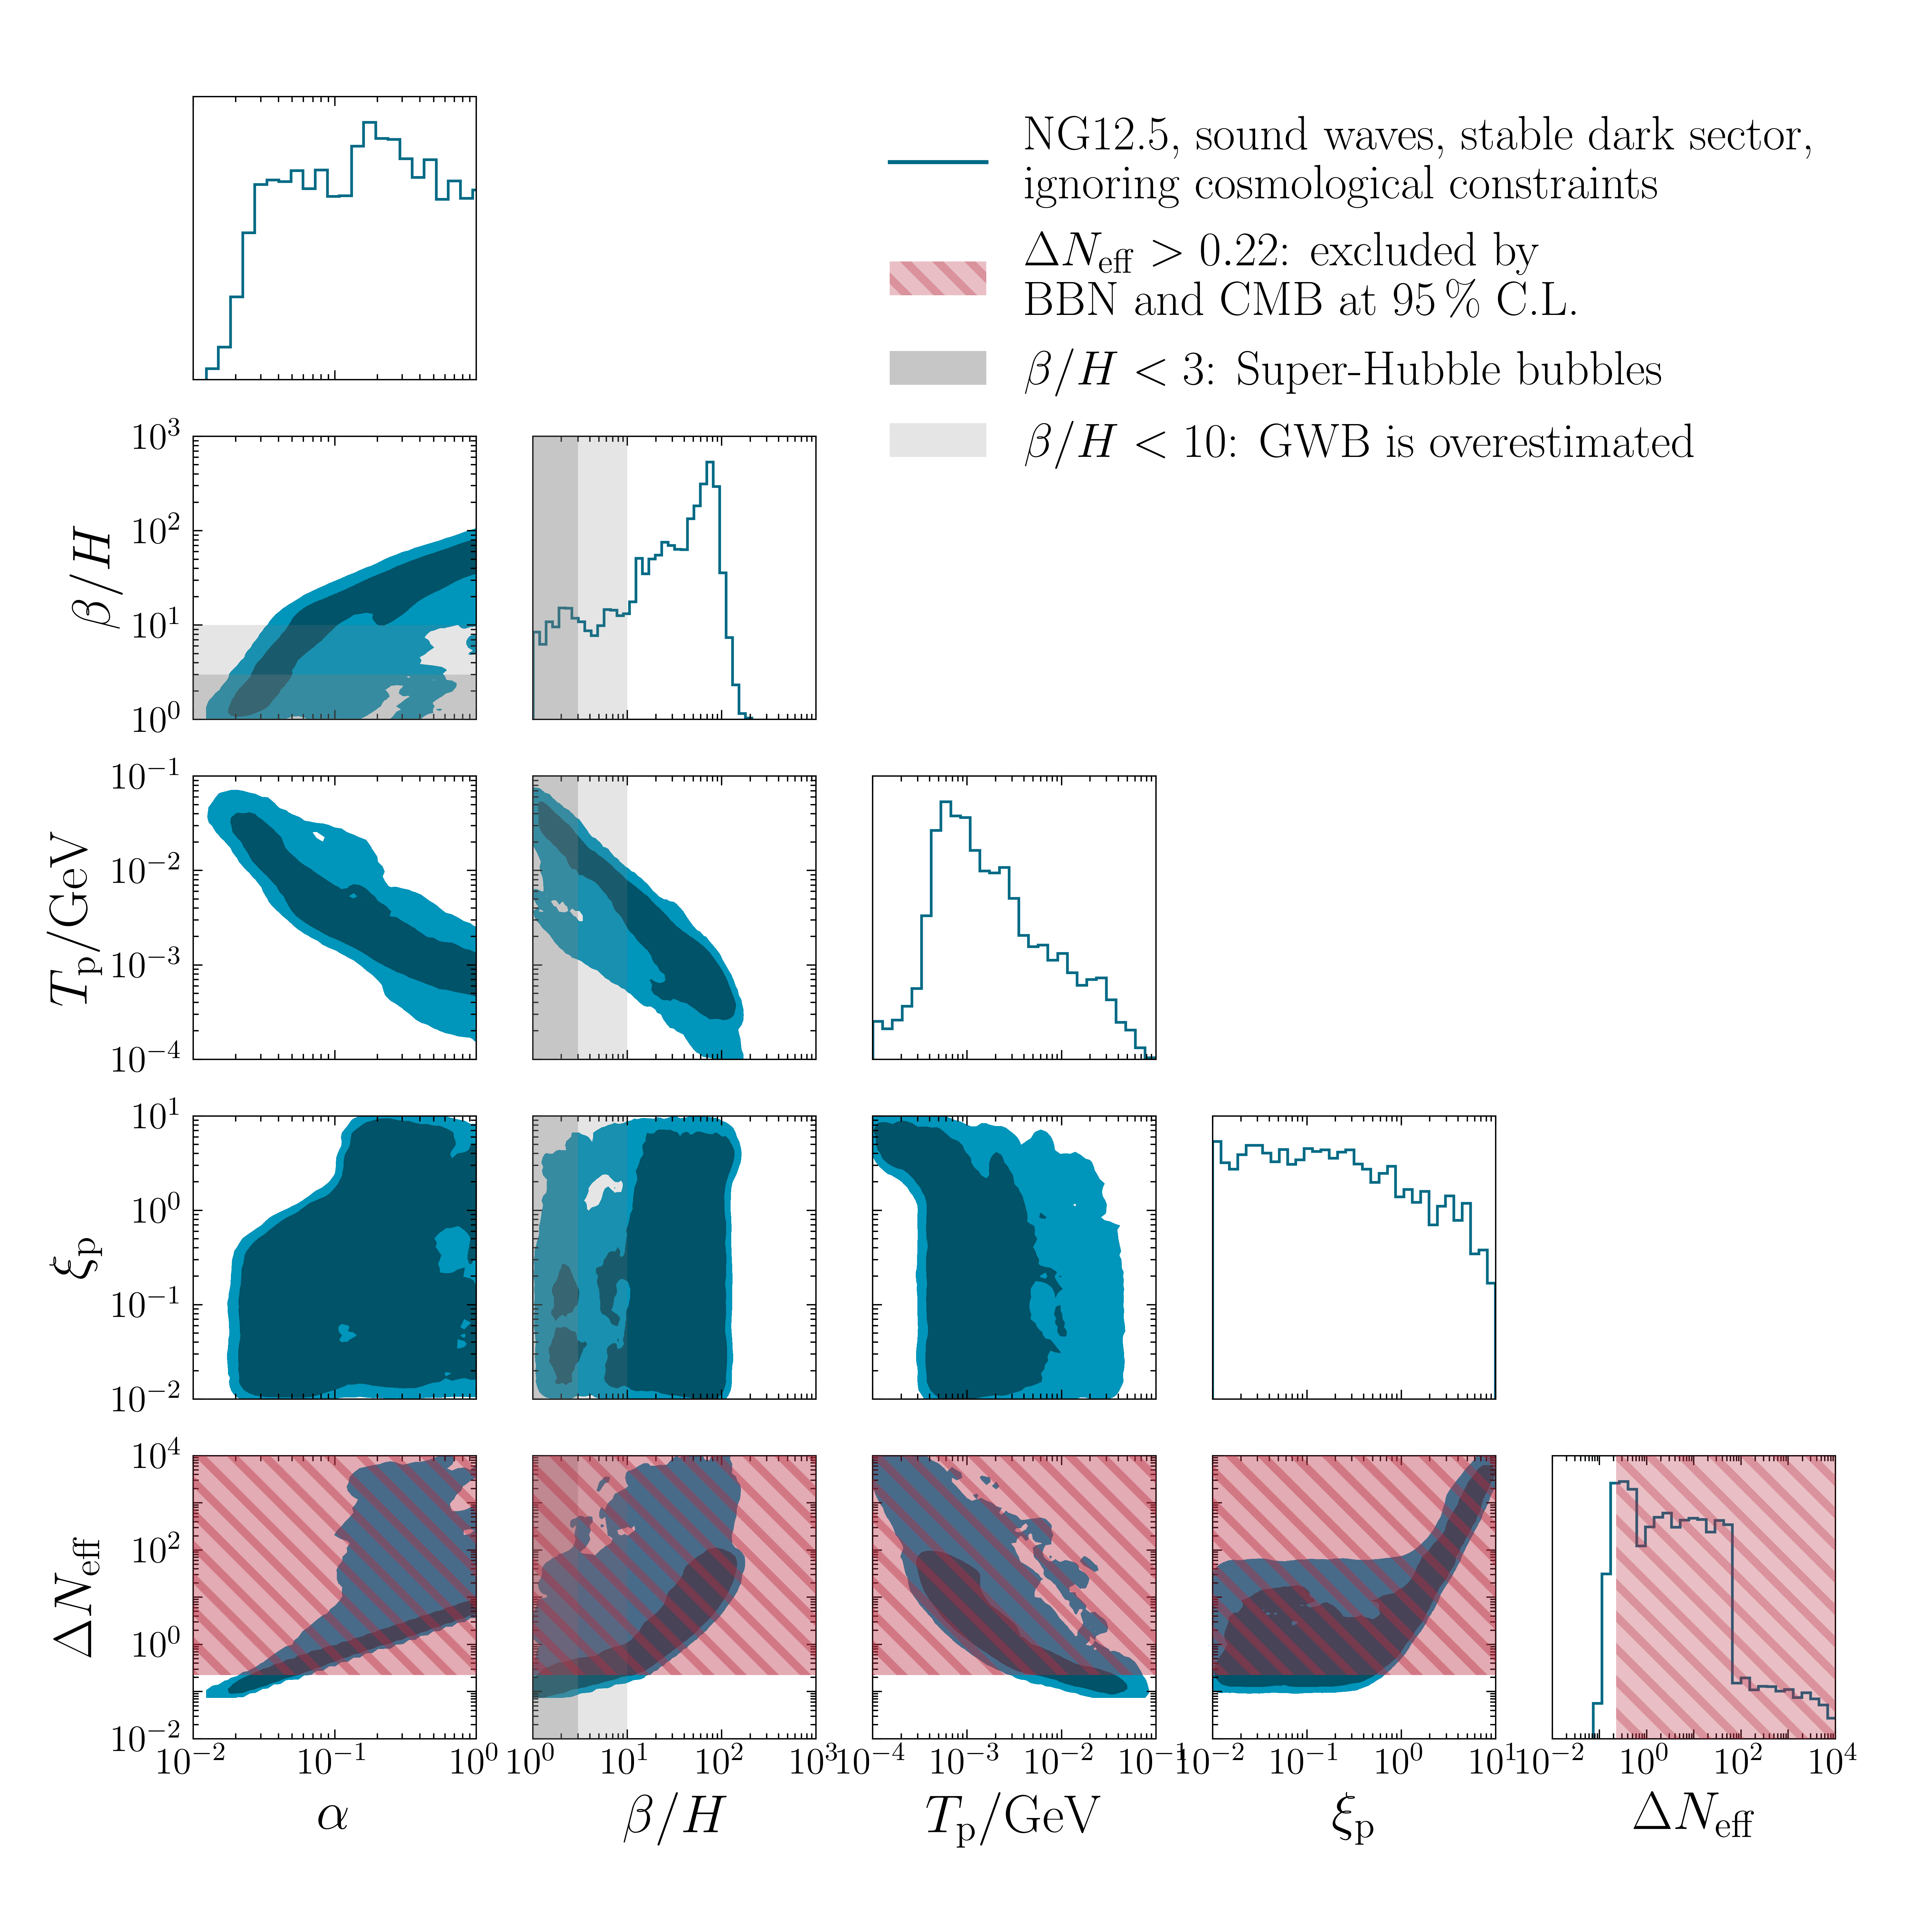
\includegraphics[width=\linewidth]{thesisplots/ptbbn/ptbbn_1}
	\caption{Triangle plot showing the $1\sigma$ and $2\sigma$ contours
		obtained by a naive fit (\textcolor{DESYdunkelblau}{blue}) of the \ac{NANOGrav} 12.5yr data to a \ac{GW} spectrum emitted in a \ac{DSPT}, ignoring cosmological constraints. To illustrate the tension with \ac{BBN} and \ac{CMB}, the 95\% C.L. excluded regions corresponding to $\Delta N_\text{eff} > 0.22$ are shaded in \textcolor{DESYdunkelrot}{red}~\cite{Yeh:2022heq}, cf.~the discussion in section~\ref{sec:constraints}. The regions in which super-Hubble bubbles ($\beta/H < 3$) and an overestimation of the \ac{GW} background amplitude ($\beta/H < 10$) are expected are shaded in \textcolor{gray}{gray}, see section~\ref{sec:spectra} for further details.}
	\label{fig:Neff_plot}
\end{figure}

Fig.~\ref{fig:Neff_plot} illustrates in a nutshell the need to consistently combine cosmological and pulsar timing information when interpreting the \ac{NANOGrav} 12.5yr results in terms of a \ac{DSPT}.\footnote{In the analysis presented in this chapter we used the now outdated \ac{NANOGrav} 12.5yr data set instead of the latest 15yr data release. We comment on expected differences between the datasets in the context of our \ac{PT} parameter inference in section~\ref{sec:results}.} The blue contours show the results of a naive fit of the \ac{DSPT} parameters to \ac{NANOGrav} data, \textit{without} taking into account physically motivated priors on the rate $\beta/H$ of the \ac{PT} or cosmological constraints.  \graffito{A first glance at the tension for stable \acp{DSPT}} We discuss the former in more detail in section~\ref{sec:spectra}, and the latter in section~\ref{sec:constraints}. Here, we simply want to demonstrate that these considerations (as indicated by gray and red shadings, respectively) will necessarily have a major impact on the naively inferred parameter space. One of our main results from a full statistical treatment, including information from cosmology, is indeed that an astrophysical explanation of the \ac{GW} signal is much more credible than a \ac{GWB} due to a \ac{PT} from a \textit{stable} \ac{DS} for sub-horizon bubble sizes $R_\ast H_\ast < 1$ (corresponding to $\beta/H \gtrsim 3$, cf.~eq.~(5.49) in ref.~\cite{Athron:2023xlk}). When considering a \ac{DS} that \textit{decays} at pre-\ac{BBN} temperatures, on the other hand, we find that the viable parameter space of \acp{DSPT} opens up: In this case, the \ac{NANOGrav} data can be explained without violating \ac{BBN} constraints, fitting the pulsar timing data as good as \acp{SMBHB}. For earlier works on cosmological constraints on \ac{PT} interpretations of the \ac{NANOGrav} results, see refs.~\cite{Nakai:2020oit,Bai:2021ibt,Deng:2023seh}.

This chapter is organized as follows: We start by discussing our parameterization of \ac{GWB} spectra from \acp{DSPT} in section~\ref{sec:spectra}. In section~\ref{sec:pta} we continue with a detailed description of our statistical procedure to analyze \ac{PTA} data, remarking also on pitfalls and limitations of simpler or more heuristic methods sometimes adopted in the literature. \graffito{Outline of this chapter} We describe the cosmological constraints on \ac{DS} dynamics  in section~\ref{sec:constraints}, and explain how to construct global likelihoods that simultaneously take into account pulsar timing and cosmological information. We present our results in section~\ref{sec:results}, before concluding in section~\ref{sec:conclusion}. In three appendices, we provide further technical details about our analysis. 

\section{Computation of GW spectra}
\label{sec:spectra}

In our analysis of the \ac{PT} interpretation of the \ac{PTA} data we use the parameterization of \acp{GWB} emitted through bubble collisions and sound waves provided in eqs.~\eqref{eq:bw} and \eqref{eq:sw}, respectively. In order to perform a data analysis that \graffito{Model-independent treatment} is as model-independent as possible, we further do not specify an underlying \ac{DS} Lagrangian, but instead infer the \ac{PT} parameters $\alpha$, $\beta/H$, $T_\perc$ and $\xi_\perc$  occurring in the semi-analytical \ac{GW} spectra in eqs.~\eqref{eq:bw} and \eqref{eq:sw} through a fit with the \ac{PTA} data. This allows us to understand the conditions a specific \ac{DS} model needs to satisfy in order to explain the nHz signal. In the following paragraphs we want to briefly summarize the assumptions that go into our parameterization of the \ac{GWB}.

We use $\xi_\perc \equiv T_\text{d,p} / T_\text{p}$ to denote the ratio of the \ac{DS} temperature in the symmetric phase to that of the \ac{SM} bath at the time of percolation. Assuming that the energy injection into the \ac{DS} bath happens instantaneously after percolation, this means that $\xi_\perc$ corresponds to the ratio just \textit{before} the \ac{PT}. To simplify our analysis, \graffito{$\xi_\mathrm{p}$: temperature ratio before the \ac{PT}} we also assume that the \ac{DS} reheats instantaneously (cf.~sec.~\ref{sec:thermalization} in the following chapter) and that the \ac{DS} energy density after the transition is dominated by at least one relativistic particle species, such that the speed of sound is given by $c_\text{s}^\text{DS} = {1}/{\sqrt{3}}$ throughout the transition.\footnote{The authors of ref.~\cite{Tenkanen:2022tly} found that a slightly smaller speed of sound is expected in the broken phase of minimal \ac{DS} models, which can lead to a sizable suppression of the \ac{GW} signal for detonations. This would introduce a model dependence which we neglect in our analysis.}

Following the example of ref.~\cite{Freese:2022qrl}, we demand $\beta/H>3$ for successful percolation. This condition can also be interpreted as requiring that the bubbles have sub-horizon size during percolation, since $R_\ast H_\ast > 1$ implies $\beta/H > \ba{8 \pi}^{1/3} = 2.93$. Moreover, the time between the nucleation of the first bubbles to \graffito{Small $\beta/H$ are problematic} percolation is about $10/\beta$ (see, e.g., ref.~\cite{Jinno:2022mie}). As simulations neglect the expansion of the Universe during the \ac{PT}, which suppresses the \ac{GW} signal, spectra obtained from such simulations are therefore likely overestimated, or at least subject to sizable uncertainties, for $\beta/H<10$. 

Concerning the exact form of the \ac{GW} spectra that we adopt here, let us mention that recent results seem to indicate sound shell decays leading to an $f^{-3}$ rather than $f^{-4}$ scaling in the \ac{UV}~\cite{Jinno:2022mie}. This scaling has little impact on our results since very low phase transition temperatures are disfavored in our analysis, \graffito{\ac{UV} tail of \ac{GWB} spectra does not matter} implying that the signal is not fitted by the (far) \ac{UV} tail. Moreover, for wall velocities close to the speed of sound, the sound shell thickness becomes imprinted in the fluid motion~\cite{Hindmarsh:2016lnk, Jinno:2020eqg, Jinno:2022mie, Hindmarsh:2019phv}. This leads to an additional knee in the power spectrum and an intermediate scaling $x^1$. We also neglect this effect since we focus on wall velocities close to the speed of light.

In all scenarios studied in this chapter, we set the dilution factor appearing in eq.~\eqref{eq:dilution} to $D = 1$, corresponding to the assumption that there is no significant deviation from the standard cosmological redshift history. This is natural in our analysis \graffito{Dilution $D$ is negligible} of stable \acp{DS}, as the potential dilution gets sourced by an entropy injection, which can only happen for decaying \acp{DS}. A dilution factor $D > 1$ would correspond to a faster expansion than in radiation domination, e.g.~if the \ac{PT} were followed by an intermediate phase of early matter domination~\cite{Ertas:2021xeh}. We checked that this dilution is always negligible also in the case of our decaying \ac{DS} scenario, cf.~appendix~\ref{app:cosmo_decaying_ds}. We find that the assumption of radiation domination (corresponding to small deviations with respect to $D = 1$) holds within the parameter space favored by the data, thereby justifying this assumption a-posteriori (see below for a discussion and appendix \ref{app:cosmo_decaying_ds} for further details).

We further set $g_{\text{DS}}^\perc = h_{\text{DS}}^\perc = 1$. This is not a strong assumption, as the \ac{DS} \acp{dof} always appear as prefactors of higher powers of  $\xi_\perc$ in the calculation. Since the experimentally preferred temperature ratios $\xi_\perc$ are small,\graffito{A specific choice for \ac{DS} \acp{dof}} corresponding to cold \acp{DSPT}, the spectrum's dependence on the precise number of \ac{DS} \acp{dof} is negligible. As discussed in section~\ref{sec:constraints}, this choice also does not influence the cosmological constraints that we impose.

Finally, we treat bubble wall collisions and sound wave spectra, parameterized in eq.~\eqref{eq:bw} and eq.~\eqref{eq:sw}, as two separate models. For bubble wall spectra, we set $\kappa_\phi = 1$ and consider only this contribution to the total \ac{GW} spectrum. For sound waves, we compute $\kappa_\sw(\alpha_\DS)$ using the high-velocity approximation from ref.~\cite{Espinosa:2010hh}, which yields $\kappa_\sw \simeq 1$ for large $\alpha_\DS$ in the case of non-runaway bubbles. \graffito{Fast dark bubble walls} Note that large $\alpha_\DS$ are generally expected due to $\alpha_\DS \propto \xi_\perc^{-4}$ in the limit of cold \acp{DSPT} $\xi_\perc \ll 1$ (cf.~eq.~\eqref{eq:alphaDS}). Hence, the conversion efficiency of vacuum energy to bulk fluid motion is generally large, $\kappa_\text{sw} \rightarrow 1$, and ultra-relativistic bubble wall velocities $\vw \rightarrow 1$ are favored by the data.

In summary, we calculate the \ac{GWB} spectrum based on the following set of \ac{DSPT} parameters:
\begin{align}
	\bc{\alpha, \beta/H, T_\perc, \xi_\perc}  .
\end{align}
In fig.~\ref{fig:spectrainfo} we illustrate the generic influence of increasing $\alpha$, $\beta/H$, and $T_\perc$ on the sound wave and bubble wall collision spectra. The influence of $\xi_\perc$ on the \ac{GWB} spectrum turns out to be negligible in our analysis \graffito{Four \ac{DSPT} parameters for the \ac{GWB}} since cosmological constraints limit it to a sufficiently small value, cf.~section~\ref{sec:results}. The spectra shown here correspond to the best-fit points of the analysis including cosmological constraints presented in section~\ref{sec:results} (with a prior of $\beta/H>1$).

\begin{figure}[t]
	\centering
	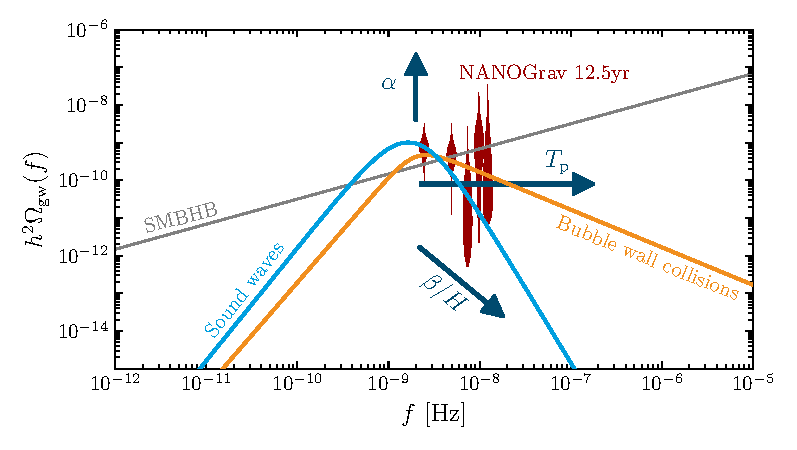
\includegraphics[width=\linewidth]{thesisplots/ptbbn/ptbbn_2}
	\caption{Plot showing the \ac{NANOGrav} 12.5yr ``violins'' (\textcolor{DESYdunkelrot}{red}) \cite{NANOGrav:2020bcs}, their standard 
		explanation through a power-law spectrum from the inspiral of \acp{SMBHB} with $A_\text{SMBHB} = 1.53 \times 10^{-15}$ and 
		$\gamma_\text{SMBHB} = 13/3$ (\textcolor{gray}{gray}), as well as two \ac{PT} spectra. A characteristic bubble wall collision spectrum is shown in \textcolor{DESYorange}{orange}. A sound wave-induced \ac{GWB} spectrum is shown in \textcolor{DESYcyan}{blue}. These spectra correspond to the best-fit parameter points found in section~\ref{sec:results} (including cosmological constraints and demanding $\beta/H > 1$). The blue arrows indicate how an increase in the \ac{PT} parameters $\alpha$, $T_\perc$ or $\beta/H$ would shift the spectra.}
	\label{fig:spectrainfo}
\end{figure}

\section{Pulsar timing array data analysis}
\label{sec:pta}

In this section, we briefly review the commonly used methods for analyzing \ac{PTA} data. We begin by discussing two approaches frequently found in the literature that are used to fit arbitrary \acp{GWB} to \ac{PTA} data. Following that, we explain in detail why  \graffito{Our global fits require \texttt{enterprise}} model comparisons based on global fits require a more rigorous analysis, specifically using the full \ac{PTA} likelihood as implemented in \ac{NANOGrav}’s code \texttt{enterprise}~\cite{enterprise, enterprise2}, cf.~eq.~\eqref{eq:PTAlikelihood}.

The \ac{NANOGrav} collaboration found that the \ac{CURN} signal (see chapter~\ref{chp:PTAs}) in their 12.5yr data set can be well-described by a power-law, cf.~eqs.~\eqref{eq:specconversion} and \eqref{eq:Phif},
\begin{align}
	h^2 \Omega_{\gw}(f) = \frac{2 \pi^2}{3 H_{100}^2} f^2 h_\text{c}^2(f) = \frac{2 \pi^2}{3 H_{100}^2} A^2  \ba{\frac{f}{1 \, \text{yr}^{-1}}}^{5 - \gamma} \text{yr}^{-2} \, , \label{eq:PTA_power_law}
\end{align}
where $A$ and $\gamma$ are the spectral amplitude and tilt, respectively. Keeping the tilt fixed to $\gamma = 13/3$ as expected for a \ac{GWB} from inspiraling \acp{SMBHB}, see section~\ref{sec:SMBHBs}, they reported a preferred signal amplitude $A \simeq 1.53 \cdot 10^{-15}$~\cite{NANOGrav:2020bcs}.

An easy-to-implement possibility to fit \textit{arbitrary} \ac{GWB} spectra to \ac{PTA} data is to reinterpret the posterior contours in the $(A, \gamma)$-plane produced by collaborations, cf.~fig.~\ref{fig:nano15astrogwcompare}, to also be \graffito{Mapping broken power-laws to $A$ and $\gamma$ is not sufficient} valid for a \ac{GWB} whose spectrum is close to a power-law in a certain frequency interval. This method has been used in many works~\cite{Freese:2022qrl, Benetti:2021uea, Blasi:2020mfx, Ellis:2020ena, Vaskonen:2020lbd, Buchmuller:2020lbh} that aim to explain the \ac{CURN} signal by a \ac{GWB} from cosmic origins rather than astrophysical sources. 
Since \acp{PT} result in \acp{GWB} with a broken power-law shape, this mapping to a specific combination of $A$ and $\gamma$ breaks down around the peak of the spectrum. While this method is often sufficient for estimating the approximate overall amplitude of the signal, it is not powerful enough for making a proper model comparison between different signal hypotheses.

Another tempting possibility to fit an arbitrary \ac{GWB} spectrum to the \ac{CURN} signal is to use the results of a free spectral analysis to the \ac{PTA} data, which lead to the infamous ``violins'' reproduced in fig.~\ref{fig:spectrainfo}. In that analysis the assumption of a power-law \ac{GWB} is dropped in favor of free spectral amplitudes at the \graffito{Using \texttt{ceffyl} would be tempting...} frequencies of integer multiples of $1/T_\text{obs}$. This approach then allows to directly fit spectra which can in principle deviate arbitrarily from a power-law (see, e.g., refs.~\cite{Ratzinger:2020koh,Wang:2022rjz, Wang:2022wwj, Ratzinger:2023umd}). This approach eventually led to \ac{NANOGrav}'s own tool \texttt{ceffyl}~\cite{Lamb:2023jls} which promises a fast evaluation of the \ac{PTA} likelihood, when marginalized over the pulsar-intrinsic red noise parameters, cf.~eq.~\eqref{eq:ceffyl}.  A significant limitation of this approach is, however, that the posteriors for the respective frequency bins are calculated with a finite prior range of signal amplitudes. Adding to the fact that the tails of these posteriors are not necessarily sampled well enough, this implies that the violins cannot be used in any statistically meaningful way for signal amplitudes too far from their most likely values. For example, the finite extent of the violins shown in fig.~\ref{fig:spectrainfo} would strictly speaking imply that the `no-signal' (i.e., the \acf{NCRN}) hypothesis is excluded with arbitrary confidence---while in reality it is only disfavored by a Bayes factor of $\sim10^4-10^5$~\cite{NANOGrav:2020bcs}!  

Crucially for our analysis, cosmological constraints can force a potential \ac{DSPT} to be so weak that the resulting \ac{GWB} spectrum contributes only negligibly to the measured \ac{CURN}. In such cases, the signal is fitted by fine-tuning the individual pulsar-intrinsic red noise amplitudes from eq.~\eqref{eq:kappaaf}. The methods discussed above implicitly rely on likelihoods that marginalize \graffito{... but leads to statistical fallacies for weak \acp{GWB}.} over these pulsar-intrinsic red noise parameters, making them unsuitable for our analysis. To properly account for correlations, a full evaluation of the likelihood is required. This approach to fitting cosmological \ac{GWB} spectra using the full \ac{PTA} likelihood has only been employed in a limited number of studies\cite{Dandoy:2023jot, NANOGrav:2021flc}, due to the high computational cost, and---to the best of our knowledge---never in a context that also incorporates additional constraining likelihoods, such as those from cosmology.

To interpret the \ac{NANOGrav} data in terms of a \ac{DSPT} we first construct a likelihood $\mathcal{L}_\text{PTA}(\bm{\theta}_\text{PSR}, \bm{\theta}_\DS)$ for fitting the timing residuals to a given set of pulsar-intrinsic red noise parameters $\bm{\theta}_\text{PSR}$ and a \ac{GW} spectrum that depends on the \ac{DSPT} parameters $\bm{\theta}_\DS$. Each pulsar's \graffito{Constructing a global likelihood} red noise is fitted by a power-law with an amplitude $A_{a}$ and slope $\gamma_{a}$, cf.~eq.~\eqref{eq:kappaaf}. To include constraints from  cosmology on the available \ac{DS} parameter space $\bm{\theta}_\DS$, we further construct a likelihood $\mathcal{L}_\text{cosmo}(\bm{\theta}_\DS)$ in section~\ref{sec:constraints}. We multiply this likelihood with the PTA 
likelihood to obtain a global likelihood,
\begin{align}
	\mathcal{L}_\text{glob}(\bm{\theta}_\text{PSR}, \bm{\theta}_\text{DS}) = \mathcal{L}_\text{PTA}(\bm{\theta}_\text{PSR}, \bm{\theta}_\DS) \times \mathcal{L}_\text{cosmo}(\bm{\theta}_\DS) \, . \label{eq:PTA_glob_lik}
\end{align}

In this analysis we concentrate on the \ac{NANOGrav} 12.5\,yr data \cite{NANOGrav:2020bcs}, for which the full set of arrival time data, the pulsar white noise parameters as well as a tutorial on how to use these resources is publicly available \cite{NANOGravTut}. In this data set, a total of 47 pulsars was taken into account, out of which we consider those that were observed for at least three years, as done in the original analysis~\cite{NANOGrav:2020bcs}. From the remaining 45 pulsars, \graffito{Analysis choices for the 12.5yr data set} we treat the pulsar J1713+0747 as advertised in ref.~\cite{NANOGravTut} due to the probably mis-modeled noise process found in the dropout analysis~\cite{NANOGrav:2020bcs}. The parameter space we evaluate therefore consists of 90 nuisance parameters $\bm{\theta}_\text{PSR} =\{ A_a, \gamma_a\} $ for the pulsar-intrinsic red noise, adding to our four (five) \ac{DSPT} model parameters $\bm{\theta}_\text{DS}$ for the case of a stable (decaying) \ac{DSPT}. To evaluate this high-dimensional global likelihood in a numerically feasible way, we implement the \ac{DSPT} spectra and $\mathcal{L}_\text{cosmo}(\bm{\theta}_\DS)$ into the codes \texttt{enterprise} and \texttt{enterprise\_extensions}~\cite{enterprise, enterprise2}. To sample over the global likelihood we use \texttt{PTMCMC}~\cite{justin_ellis_2017_1037579}. The \ac{MCMC} chains are evaluated using \texttt{numpy} and \texttt{scipy}~\cite{Virtanen:2019joe}, and triangle plots are generated using \texttt{matplotlib} and a customized version of \texttt{ChainConsumer}~\cite{Hinton2016}. For performing model comparisons, finally, we calculate Bayes factors using the product space method~\cite{Hee:2015eba,10.2307/1391010, Chamberlin:2014ria, 10.2307/2346151}, which we briefly review in appendix~\ref{sec:product_space_method}.

\section{Cosmological constraints}
\label{sec:constraints}

The past decades of observational cosmology have provided a large amount of data which allow us to confidently reconstruct the cosmological evolution up to MeV-scale temperatures. Most notably these include observations of the CMB, both in terms of the spectral shape~\cite{Fixsen:1996nj} and anisotropies~\cite{Planck:2018vyg}, and the primordial light element abundances produced during \ac{BBN}~\cite{ParticleDataGroup:2022pth}. These observations are \graffito{Precision cosmology at the MeV-scale} in very good agreement with the standard \ac{LCDM} model and with each other~\cite{ParticleDataGroup:2022pth}, implying that any changes to \ac{LCDM}  at temperatures below a few $\mathrm{MeV}$ can have observational consequences and need to be checked for consistency with available \ac{CMB} and \ac{BBN} 
data~\cite{Planck:2018vyg,Hufnagel:2018bjp,Forestell:2018txr,Depta:2020zbh,Depta:2020mhj,Kawasaki:2020qxm,Yeh:2022heq}.

For a \ac{PT} to produce a strong \ac{GW} signal a sizable amount of vacuum energy needs to be released in the transition, most of which is subsequently converted into \ac{DS} energy density as only a small fraction ends up in the \ac{GWB}. This additional energy density could change the well-tested cosmic expansion history, possibly even long after the transition itself. \graffito{BBN and CMB constraints are most important} To understand whether \acp{PTA} may observe the remnants of such a \ac{PT} we therefore need to include a cosmological likelihood $\mathcal{L}_\text{cosmo}$ when analyzing the \ac{PTA} data. Specifically, we include information from the primordial light element abundances and \ac{CMB} anisotropies into our analysis as described below.\footnote{Note that constraints from $\mu$-distortions of the \ac{CMB} photon spectrum~\cite{Ramberg:2022irf} and curvature perturbations~\cite{Liu:2022lvz} are less relevant as they quickly lose sensitivity for transition temperatures above the MeV-scale. \ac{PBH} formation due to first-order phase transitions~\cite{Lewicki:2023ioy,Gouttenoire:2023naa,Baker:2021nyl} could offer novel probes, but turns out to be irrelevant for the phase transition strengths of interest in this analysis.}

\subsection{Stable dark sectors}

If the entire \ac{DS} energy density after the \ac{PT} is contained in light degrees of freedom, this contributes an additional radiation energy density that can be described by a (potentially large) additional contribution $\DNeff$ to the effective number of neutrinos $N_\text{eff} = N_\text{eff}^\text{SM} + \DNeff$, where $N_\text{eff}^\text{SM} = 3.044$~\cite{Bennett:2020zkv} is the \ac{SM} prediction for \ac{LCDM} cosmology.\footnote{\label{foot_noMD}The assumption of a radiation-dominated \ac{DS} is conservative in the sense that constraints only become tighter if the energy density instead starts to redshift as matter at some time after the phase transition. We also note that the contribution to $\DNeff$ from the \acp{GW} themselves, for a \ac{GWB} with peak amplitude $h^2 \Omega_\text{GW}^\text{peak} \lesssim 10^{-9}$ as required to explain the \ac{NANOGrav} signal, is typically less than $\DNeff \simeq 10^{-3}$, cf.~ref.~\cite{Maggiore:2018sht}, and therefore irrelevant in the discussion of cosmological constraints.} \graffito{Stable \acp{DS} are constrained through $\Delta N_\mathrm{eff}$} The effective number of neutrinos affects the predictions of \ac{BBN} (see sec.~\ref{sec:BBN}) as well as the \ac{CMB} power spectrum and is constrained by observations to $N_\text{eff} = 2.941 \pm 0.143$~\cite{Yeh:2022heq}. This bound can be modeled by a Gaussian likelihood $\mathcal{L}_{\text{BBN} + \text{CMB}} (N_\text{eff})$, i.e.
\begin{align}
	\mathcal{L}_\text{cosmo} (\bm{\theta}_\DS) = \mathcal{L}_{\text{BBN} + \text{CMB}} (N_\text{eff} = N_\text{eff}^\text{SM} + \DNeff(\bm{\theta}_\DS))\,,
\end{align}
enabling us to implement the cosmological constraints for the case of a stable \ac{DS}. The number of \acp{dof} in the \ac{DS} does not have any relevant impact on cosmological constraints as the available latent heat would simply be distributed among the different species, leaving the total injected energy density unchanged. (Taking into account the energy density \emph{before} the phase transition, a change in the number of \acp{dof} can be absorbed in the temperature ratio $\xi_\mathrm{d}$ which we treat as a free parameter in our scans anyway.) We therefore set $g_{\DS}^\perc=1$ in our analysis. For more details we refer to appendix~\ref{app:cosmo_stable_ds}.

\subsection{Decaying dark sectors}
If there are additional small inter-sector couplings---which happens very naturally due to possible `portal' couplings such as Higgs mixing for scalars or kinetic mixing for dark photons---the energy density injected into the \ac{DS} will subsequently be \graffito{Decaying \ac{DS} constraints depend on the mediator's mass and lifetime} transferred to the \ac{SM} heat bath via decays of \ac{DS} particles. In this case cosmological constraints in general depend on the lifetime, mass, and coupling structure of the decaying particles. As a simple concrete example and for minimality, we consider the \ac{DS} after the \ac{PT} to consist only of one bosonic \ac{dof} $\phi$ decaying into photons or electrons with a lifetime $\tau_\phi$ that we sample over. This is a natural setup in the context of a potential \ac{PT} at MeV temperatures, as a light scalar \ac{dof} with mass below the \ac{PT} temperature is generally expected to exist in that case and, e.g., constraints from Higgs mixing would not be very severe.

Given that the \ac{NANOGrav} data prefer an MeV-scale \ac{PT} temperature, also the mass of $\phi$ is expected to be of this order, $m_\phi \simeq \mathrm{MeV}$. In the example of Higgs mixing very short lifetimes $\tau_\phi$ correspond to a sizable Higgs mixing angle $\theta$ \graffito{$\tau_\phi \lesssim 0.1 \, \mathrm{s}$ } which is constrained by a number of laboratory experiments to be $\theta \lesssim 10^{-4}$ for small masses~\cite{Winkler:2018qyg,Ferber:2023iso}. Translating this constraint for MeV-scale masses into the lifetime results in $\tau_\phi \gtrsim 10^{-2} \, \mathrm{s}$ whereas cosmological constraints roughly require $\tau_\phi \lesssim 10^{-1} \, \mathrm{s}$,  so that some allowed region remains even in this scenario.\footnote{Note that the case of a Higgs-mixed scalar is particularly constrained because of the Yukawa-suppressed couplings to electrons, implying a rather long lifetime. If the relevant state would be e.g.~a dark photon, the allowed range of lifetimes would be significantly larger.} As already indicated, the resulting cosmological constraints largely depend on the lifetime $\tau_\phi$ of the particle, with only a very mild dependence on the mass as long as the energy density in $\phi$ is not very suppressed. MeV and smaller masses, on the other hand, generally lead to strong constraints for arbitrarily short lifetimes $\tau_\phi$ due to thermalization by inverse decays. To simplify our analysis we therefore fix the mass of the decaying particle to $m_\phi = 5 \, \mathrm{MeV}$, noting that the results will be very similar for other choices of the mass in the MeV-range. To implement the cosmological constraints, we use a likelihood $\mathcal{L}_{\text{BBN} + \text{CMB}}$ incorporating the results from refs.~\cite{Depta:2020zbh,Bai:2021ibt} (see appendix~\ref{app:cosmo_decaying_ds} for details).


\section{Results}
\label{sec:results}

We now present the results of our data analysis, based on global fits of the model setups described in the previous sections. We begin by examining \acp{PT} in stable \acp{DS} (section~\ref{sec:results_stable}), followed by a discussion of a decaying \ac{DS} that thermalizes with the visible sector some time after the \ac{PT} (section~\ref{sec:results_decay}). Finally, we compare with the \ac{SMBHB} explanation of the signal in terms of the respective Bayes factors (section~\ref{sec:results_comp}) and explore how later \ac{PTA} data sets impact the \ac{DSPT} interpretation.

\subsection{Stable dark sector phase transitions}
\label{sec:results_stable}

Let us first focus on \acp{GW} that are mainly emitted as a consequence of the bulk motion of the \ac{DS} plasma after the \ac{PT}, i.e.~a \ac{GWB} dominantly \graffito{First: Stable \ac{DS}, \ac{GWB} from sound waves} produced through sound waves. The full set of model parameters  to describe such a scenario for a stable \ac{DSPT}, as introduced in section~\ref{sec:spectra}, is given by
\begin{align}
	\{\alpha, \beta/H, T_\perc, \xi_\perc\}\,.
\end{align}
We sample over these input parameters with flat log priors, as well as over 90 nuisance parameters $\bm{\theta}_\text{PSR}$ for the pulsar-intrinsic red noise, based on the combined \ac{PTA} and cosmological likelihood given in eq.~\eqref{eq:PTA_glob_lik}. For a full overview over parameters and prior ranges, see also table~\ref{tab:priors} in appendix~\ref{sec:priors}. 

\begin{figure}[t]
	\centering
	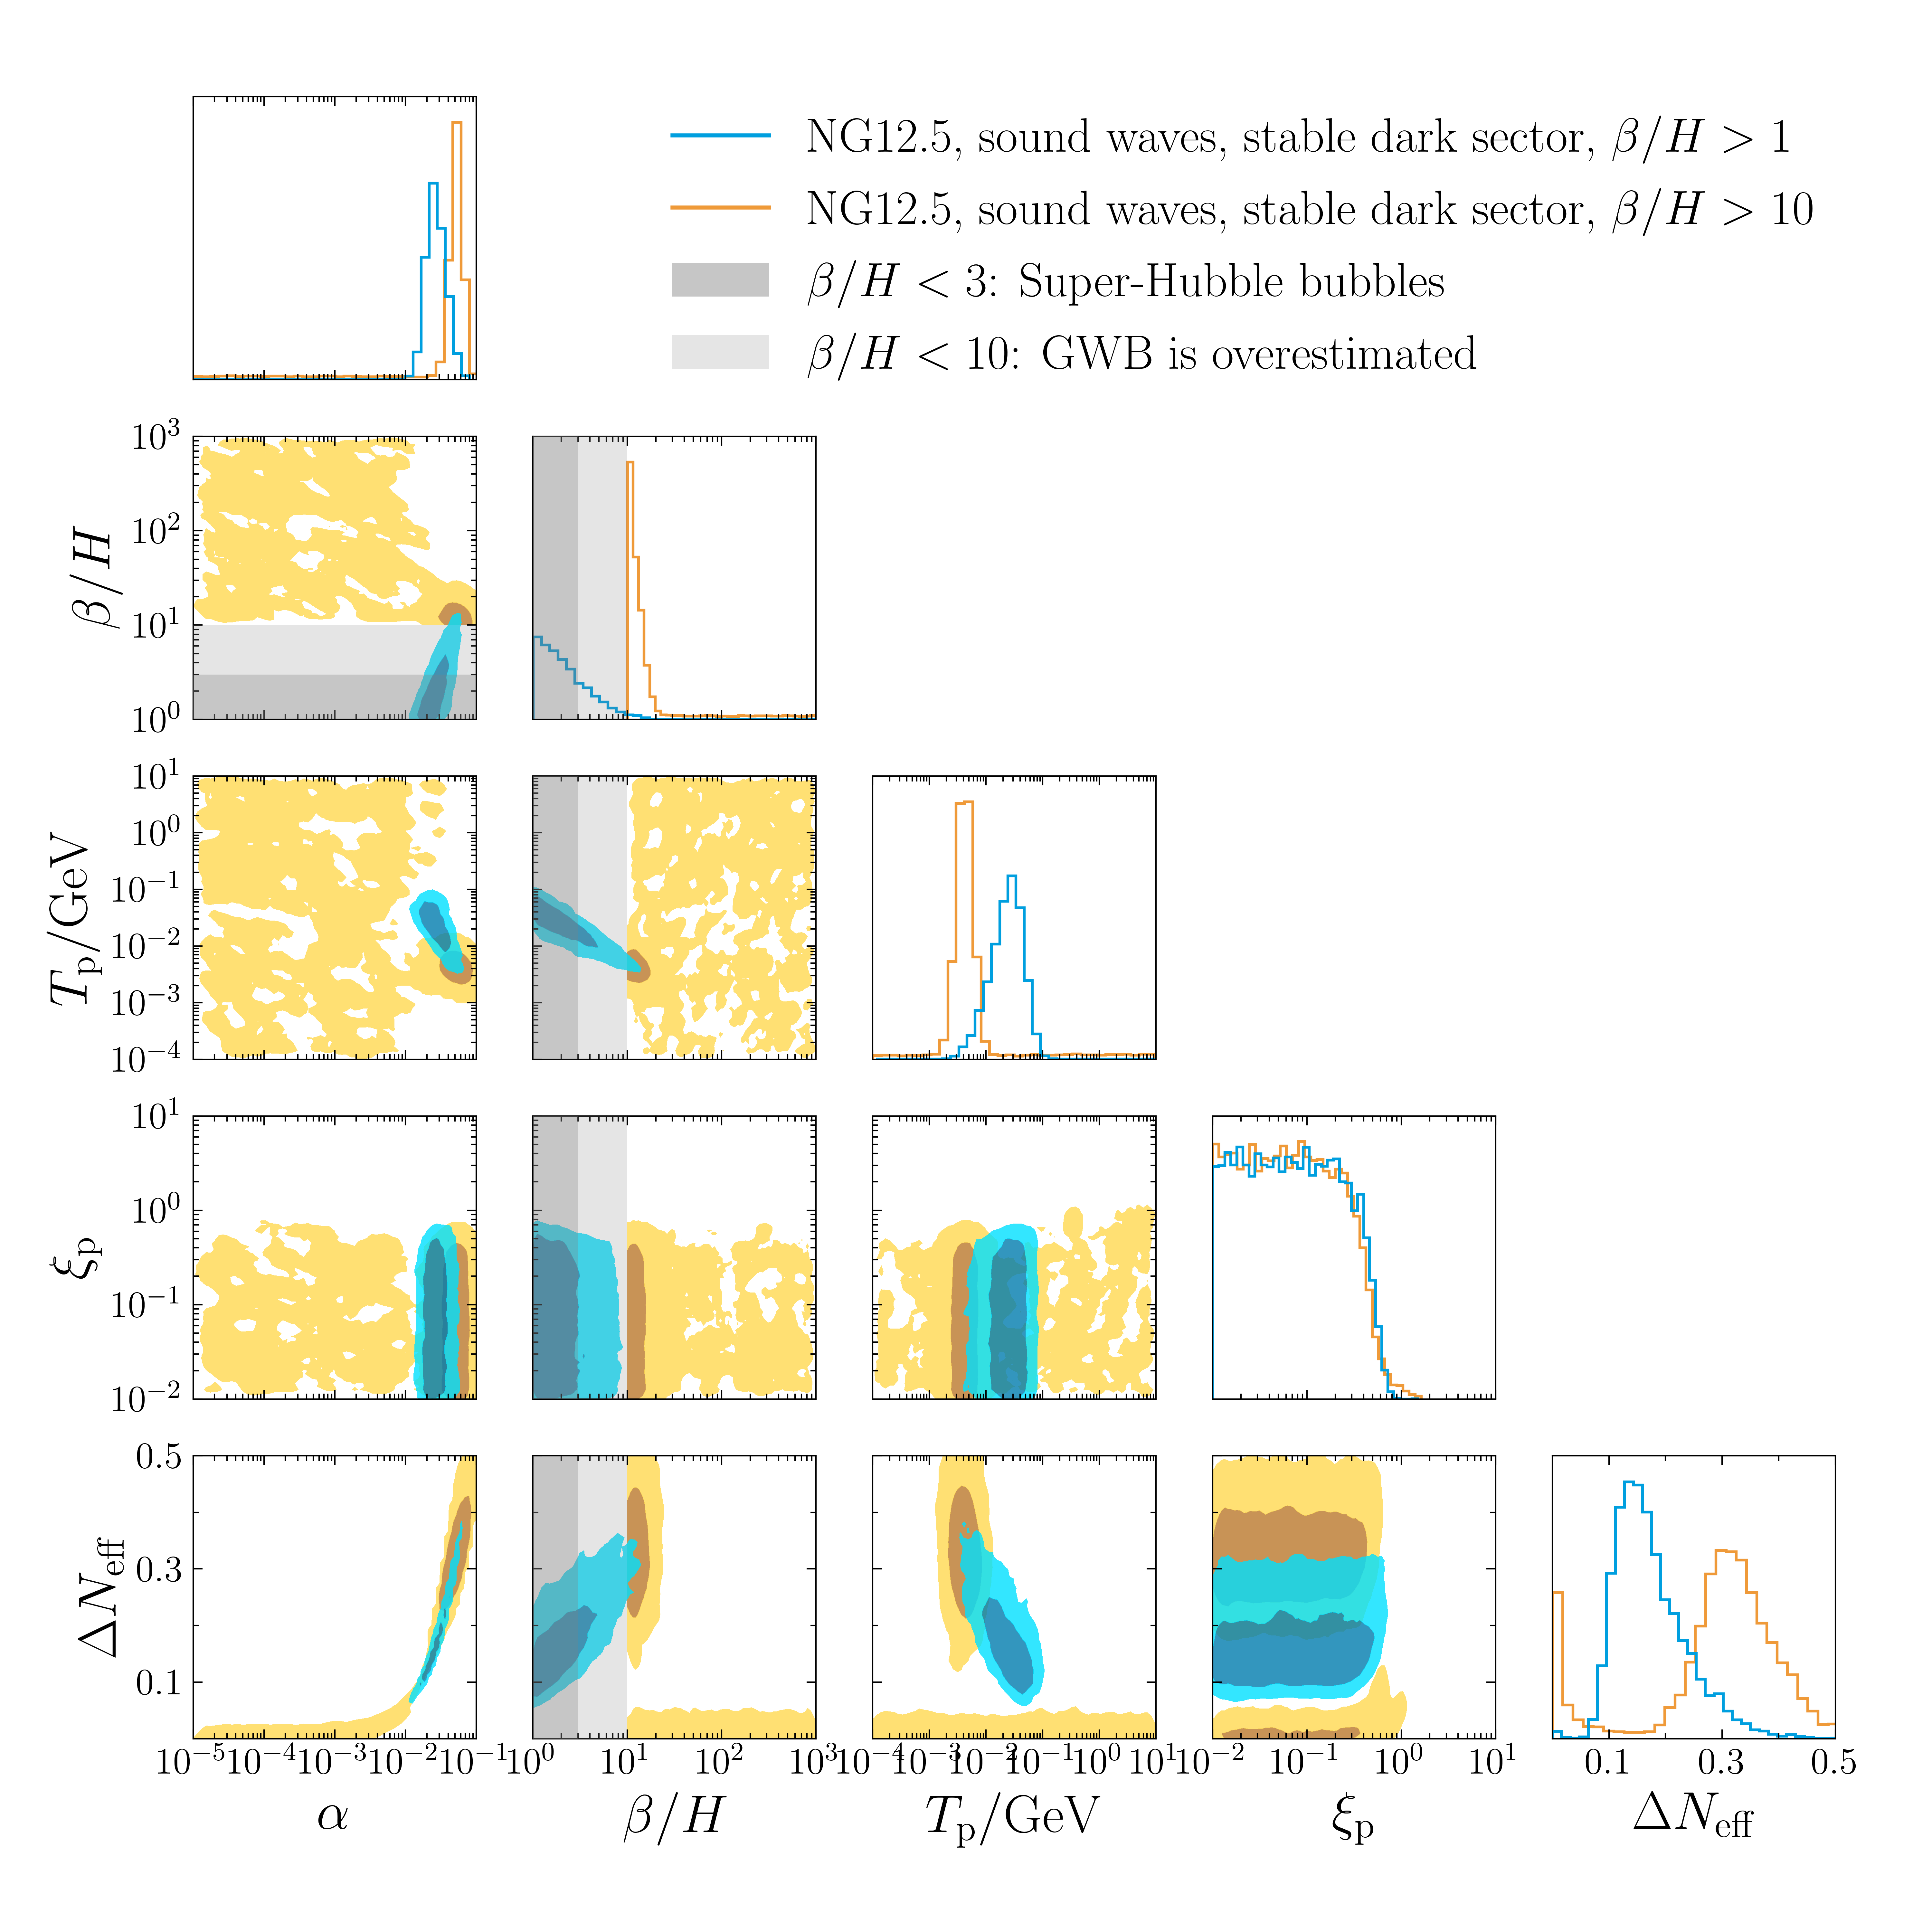
\includegraphics[width = \textwidth]{thesisplots/ptbbn/ptbbn_3}
	\caption{Comparison of the triangle plots for two \ac{MCMC} chains with different priors on $\beta/H$, assuming a stable \ac{DS} and a \ac{GWB} generated through sound waves. The shaded regions mark $1\sigma$ and $2\sigma$ contours, respectively. Regions with $\beta/H<3$ and $\beta/H<10$, in which the phase transition cannot complete and the \ac{GW} signal is overestimated respectively, are indicated with \textcolor{gray}{gray} shadings.} 
	\label{fig:tringle-comparison}
\end{figure}

We show the resulting  corner plot of posterior distributions for the four model parameters in fig.~\ref{fig:tringle-comparison}, to which we  add the derived parameter $\DNeff$. Allowing for inverse time scales down to $\beta/H > 1$ (\textcolor{DESYcyan}{light blue}) formally results in a good global fit of the pulsar timing residuals, as indicated by the compact \graffito{A seemingly good fit for $\beta/H>1$} ellipsoid-like posterior regions  where the \ac{NANOGrav} signal is explained by the \ac{GWB}.  Such small values of the transition rate would however suppress the \ac{GW} spectrum w.r.t.~the commonly adopted parameterization, cf.~the discussion in section~\ref{sec:spectra}, and, for $\beta/H \lesssim 3$, likely not even lead to successful percolation.

We therefore also show, in the same figure, the results of a fit with a more restrictive prior of $\beta/H > 10$ (\textcolor{DESYorange}{orange}).  In this case, the best-fit region moves to somewhat larger values of $\alpha$, but it also becomes apparent that there is no \graffito{For $\beta/H>10$: No single preferred best fit region} longer a single preferred region in the model parameter space: Instead, the combined data now shows a similar preference for a very weak \ac{DSPT}-induced \ac{GW} signal with correspondingly weak cosmological constraints, where the \ac{NANOGrav} signal is not explained by the \ac{GWB} but absorbed in the pulsar-intrinsic noise amplitudes $A_a$. This indicates that also the best-fit region no longer corresponds to an equally plausible interpretation of the combined data set.

The reason is that cosmology adds a constraint on $\DNeff$ which effectively translates into a constraint on the \ac{PT} strength $\alpha$. In terms of fitting the  \ac{NANOGrav} signal, the required lower value of $\alpha$ can partially be compensated by a lower value of $\beta/H$ (see also fig.~\ref{fig:spectrainfo}). And indeed, comparing the posterior distributions for $\beta/H$ in fig.~\ref{fig:tringle-comparison}, we can see that $\beta/H$ always sticks closely to the lower prior boundary---which is qualitatively different from the analysis without cosmological constraints, cf.~fig.~\ref{fig:Neff_plot}, where inverse timescales of $\beta/H = \mathcal{O}(10-100)$ are favored. Increasing the lower prior bound on $\beta/H$ therefore  directly induces a shift towards larger $\alpha$. At the same time, a larger inverse timescale $\beta/H$ also means smaller bubbles at the time of their collision, \graffito{Low $\Delta N_\mathrm{eff}$ requires low $\alpha$, $\beta/H$ and $\xi_\mathrm{p}$} and hence a larger peak frequency in the spectrum (see again fig.~\ref{fig:spectrainfo}). This is compensated for by a  lower percolation temperature $T_\perc$, which by itself would lead to smaller peak frequencies. Finally, we can identify  in fig.~\ref{fig:tringle-comparison} an upper bound on the initial  temperature ratio, which again is a direct consequence of the constraint on $\DNeff$. For $\xi_\perc \gtrsim 0.7$, in particular, eq.~\eqref{eq:Neff} would imply a violation of this constraint already for a single \ac{DS} species that is not non-relativistic before the transition~\cite{Breitbach:2018ddu}.

Overall, these effects push the posterior for $\DNeff$ towards higher values. Since this is strongly punished by the cosmological part of the likelihood, however, that also explains the already mentioned appearance of a second preferred parameter region, characterized by a weak \ac{DSPT} that corresponds to $\DNeff \simeq 0$ (at the price of an unobservably small \ac{GW} signal). \graffito{For $\Delta N_\mathrm{eff} \simeq 0$, signal is absorbed by $\{A_a, \gamma_a\}$} We confirmed that this region of parameter space is indeed explained by fine-tuning the pulsar-intrinsic red noise parameters, rather than by a \ac{GWB}, by directly comparing the marginalized posteriors of the nuisance parameters $\bm{\theta}_\text{PSR}$ between the two chains depicted in \textcolor{DESYcyan}{light blue} and \textcolor{DESYorange}{orange}. Let us stress that this parameter range would have been impossible to reliably infer with simpler statistical methods, i.e.~by re-fitting a power-law common red spectrum described by $\ba{A, \gamma}$ or by using the free-spectrum ``violins'' (see the discussion in section~\ref{sec:pta}).

\begin{figure}[t]
	\centering
	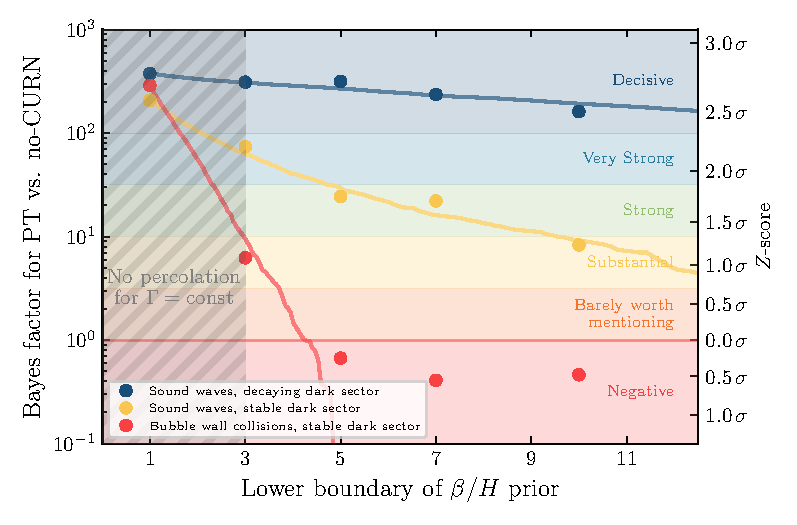
\includegraphics[width = \textwidth]{thesisplots/ptbbn/ptbbn_4}
	\caption{Bayes factor estimates of various \ac{DSPT} models with respect to the no common red noise-hypothesis. Filled colored dots correspond to actually performed full model comparisons, while lines in the corresponding colors are derived from an \textit{a posteriori} reduction of the prior range of chains with minimal $\beta/H$ of 1 (for details, see appendix~\ref{sec:priorchoice}). We also indicate how to translate the Bayes factor to  Jeffrey's scale (colored shadings) as well as $Z$-scores from frequentist statistics (right $y$-axis, cf.~appendix~\ref{sec:z-scores}). In the gray shaded area ($\beta/H < 3$), a constant nucleation rate is not sufficient to drive percolation.}
	\label{fig:BFs}
\end{figure}

From the above discussion, one would expect the Bayes factor between the \ac{DSPT} and the \ac{NCRN} hypothesis to decrease when increasing the lower prior bound on $\beta/H$, as higher and higher values of $\DNeff$  are needed to explain the combined data. We confirm this expectation explicitly in fig.~\ref{fig:BFs}. Here, each of the colored dots \graffito{Evidence for \ac{DSPT} depends on $\beta/H$ prior} corresponds to a separate \ac{MCMC} chain that was employed to determine the Bayes factor between the two models by using the product space method explained in appendix~\ref{sec:product_space_method}. The corresponding lines serve as a cross-check for the prior dependence of the Bayes factors, see appendix~\ref{sec:priorchoice} for further details. Yellow dots and lines refer to the case of a stable \ac{DSPT} where the \ac{GWB} production is dominated by sound waves; this corresponds to the same model as shown in fig.~\ref{fig:tringle-comparison}.

For comparison, we also show the case of a \ac{GWB} that is mostly due to bubble wall collisions (red). Just from the point of view of the resulting spectrum, cf.~fig.~\ref{fig:spectrainfo}, one might expect that this could be a viable alternative. \graffito{Bubble wall collisions suffer from additional $\beta/H$ suppression} Compared to sound waves,  however, bubble wall spectra receive an additional parametric suppression of $h^2\Omega_\text{GW}^\text{peak}$  by a factor of $\ba{\beta/H}^{-1}$. This induces the need for a larger $\alpha$ and hence an even stronger constraint on $\DNeff$, making the \ac{GWB} hypothesis worse than the \ac{NCRN} assumption for $\beta/H\gtrsim5$. To further illustrate these considerations, we refer to fig.~\ref{fig:spec-comparison} in appendix~\ref{sec:posteriorGWBdist}, showing the posterior distribution of the bubble wall spectra for different prior choices on  $\beta/H$. Note also that neither fig.~\ref{fig:tringle-comparison} nor fig.~\ref{fig:BFs} includes the expected suppression in the \ac{GWB} spectra for $\beta/H\lesssim10$, which would further decrease our Bayes factor estimates.

Overall we therefore come to the conclusion that a stable \ac{DSPT} can hardly compete with the alternative \ac{SMBHB} explanation of the \ac{PTA} \graffito{Stable \acp{DSPT} are in strong tension with \ac{BBN} and \ac{CMB}} timing residuals, once one takes into account cosmological constraints from \ac{BBN} and \ac{CMB}. For $\beta/H>10$, in particular, the Bayes factor between a \ac{DSPT} explanation and the \ac{NCRN} hypothesis is only $\mathcal{O}(10)$ even in the favorable case of sound wave-induced \acp{GWB}---much smaller than the factor of $\sim10^{4.5}$ that is claimed for a \ac{GWB} from \acp{SMBHB}~\cite{NANOGrav:2020bcs}. 


\subsection{Decaying dark sector phase transitions}
\label{sec:results_decay}
We next consider a \ac{DS} that couples sufficiently strongly to ordinary matter such that it can decay after the \ac{PT}. A decay long before \ac{BBN}, in particular, is not subject to the cosmological constraints that played such a decisive role for the case of a stable \ac{DSPT}. On the other hand, a \ac{PT} happening too early would produce a \ac{GWB} at too high frequencies to \graffito{Can the \ac{DS} decay before \ac{BBN}?} be compatible with the \ac{NANOGrav} signal. It is therefore a non-trivial question whether any relevant parameter space remains where \ac{PTA} and cosmological data are indeed compatible. For concreteness, we assume the decay of a dark Higgs boson as detailed in section~\ref{sec:constraints} that decays with a lifetime $\tau_\phi$, such that our model parameters read 
\begin{align}
	\{\alpha, \beta/H, T_\perc, \xi_\perc, \tau_\phi\} \, .
\end{align}
For the dark Higgs lifetime we adopt a log prior ranging from $10^{-6}\, \text{s}$ to $10^2 \, \text{s}$; the remaining parameters we treat as in the previous section (with $\beta/H>1$).

\begin{figure}[t]
	\centering
	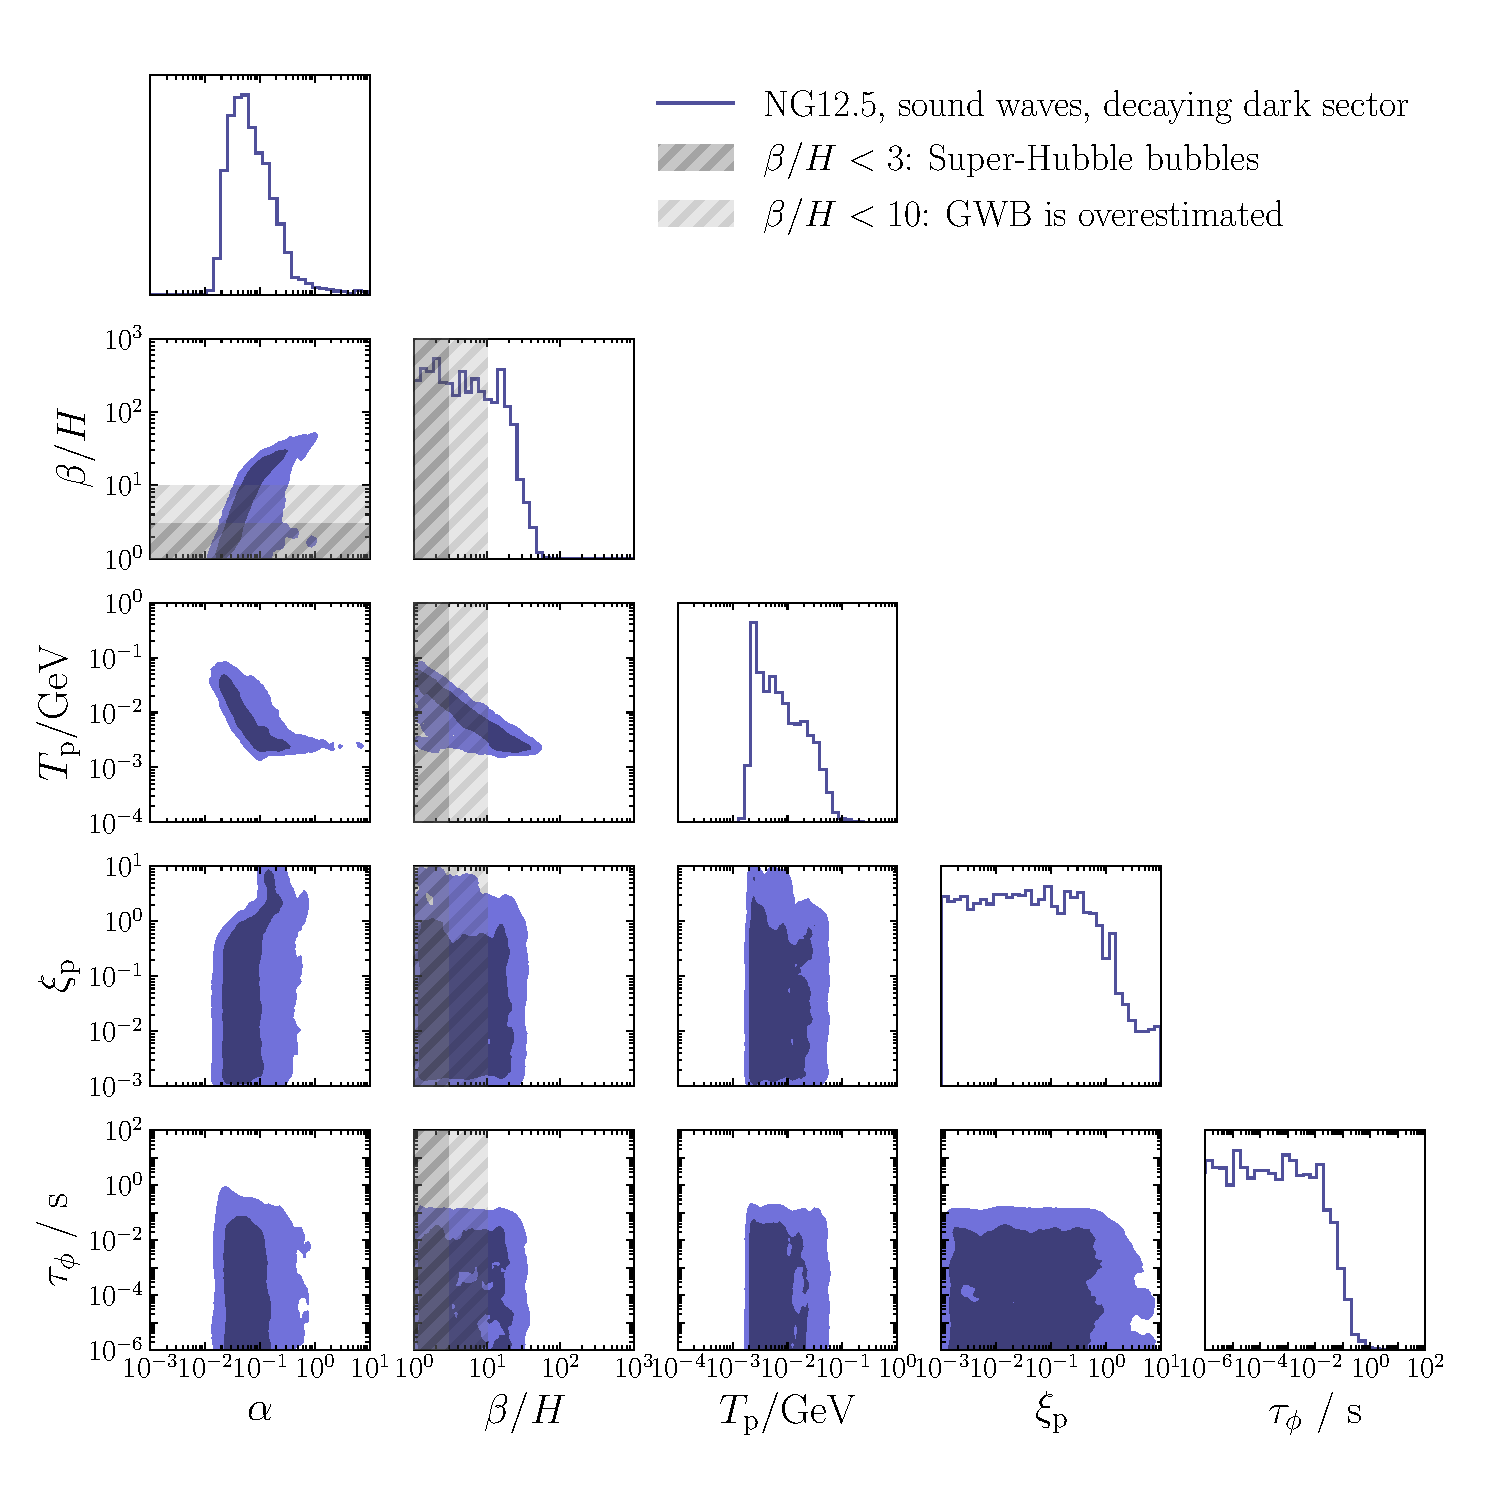
\includegraphics[width=\linewidth]{thesisplots/ptbbn/ptbbn_5}
	\caption{Posterior distributions of model parameters in the decaying dark sector scenario.}
	\label{fig:dsdecay_logprior}
\end{figure}

We show the resulting triangle plot for this model in fig.~\ref{fig:dsdecay_logprior}. In a nutshell, we find that the \ac{GW} spectrum observed by \ac{NANOGrav} can be \graffito{The decay requires $\tau_\phi \lesssim 0.1 \, \mathrm{s}$ and $T_\mathrm{p} \gtrsim 2 \, \mathrm{MeV}$}  explained as long as $\tau_\phi \lesssim 0.1 \, \text{s}$ and $T_\perc \gtrsim 2 \, \text{MeV}$. Larger lifetimes, corresponding to temperatures smaller than $2\,\text{MeV}$, are strongly constrained as the decays occur after the onset of \ac{BBN} or neutrino decoupling. Such decays change the time-temperature relation of the \ac{SM} heat bath and alter the ratio of the neutrino and photon temperatures, leading to a \textit{negative} contribution to $\DNeff$. If the percolation temperature $T_\perc$ drops to values close to the temperature of neutrino decoupling, strong constraints arise independent of the lifetime $\tau_\phi$. Note that we implemented the results from ref.~\cite{Bai:2021ibt} for simplicity as a sharp cut-off enforcing $T_\perc>2 \, \text{MeV}$ in our likelihood, cf.~appendix~\ref{app:cosmo_decaying_ds}. Adopting a more accurate likelihood would result in a smoother transition of the posterior in the range $T_\mathrm{p} \approx 1 - 2 \, \text{MeV}$, the main effect being a slight increase of the maximal possible value of $\beta / H$.

Compared to our analysis of stable \acp{DSPT}, the posterior for the inverse timescale $\beta/H$ is relatively flat up to $\beta/H\sim30$, implying a very limited prior dependence. The underlying reason for this is  the possibility of dumping the liberated energy density into the \ac{SM} photon bath before the neutrino decoupling at  around $2 \, \text{MeV}$, thereby evading \graffito{The \ac{DSPT} cannot be arbitrarily strong} cosmological constraints and hence opening up for large \ac{PT} strengths $\alpha \gtrsim0.1$ to fit the \ac{GW} signal even for $\beta/H \gtrsim 10$. This however only works up to the point when $\beta/H$ becomes so large that its effect on the peak frequency can no longer be compensated for by a correspondingly lower percolation temperature, cf.~fig.~\ref{fig:spectrainfo}.

In fig.~\ref{fig:BFs} we also indicate the Bayes factor for the decaying \ac{DSPT} scenario (blue). As anticipated, the prior dependence on $\beta/H$ is much less \graffito{``Decisive'' evidence for decaying \ac{DSPT}} severe than in the scenarios discussed previously. In particular, this shows that a \ac{GWB} from a decaying \ac{DSPT} is a viable explanation of the observed signal even for $\beta/H > 10$. Quantitatively, the model evidence is a factor of $\sim200$ larger than that of the \ac{NCRN} hypothesis, corresponding to $2.5 \sigma$ or a ``decisive'' evidence on Jeffrey's scale.


\subsection{Comparison with SMBHBs and later data sets}
\label{sec:results_comp}

Let us next address in more detail the question of how a \ac{DSPT} interpretation of the signal compares to alternative \ac{GWB} hypotheses, in particular the leading astrophysical explanation of an \ac{SMBHB}-induced \ac{GWB}, and how future data will help to further distinguish these two.

We start by pointing out that the \ac{DSPT} spectra actually fit the \ac{GW} spectrum in the \ac{NANOGrav} data slightly \textit{better} \graffito{A better fit despite smaller Bayes factors} than the \ac{SMBHB} spectra. Naively, this is already expected from fig.~\ref{fig:spectrainfo}, and we demonstrate this in more detail in appendix~\ref{sec:priorsDSPT}. Nevertheless the maximal Bayes factor (with respect to \ac{NCRN}) that we find is only about $10^{2.5}$, significantly smaller than the $\sim10^{4.5}$ typically quoted for \acp{SMBHB}~\cite{NANOGrav:2020bcs}. We checked explicitly that the reason is \textit{not} connected to the goodness-of-fit, but entirely due to prior volume effects: Bayesian statistics dutifully renders the simple \ac{SMBHB} explanation of the data more credible than the apparently more complicated \ac{DSPT} model.

However, it is important to remember that the amplitude $A_\text{SMBHB}$ of the astrophysical signal is not necessarily a single fundamental parameter, as assumed in deriving a Bayes factor of $10^{4.5}$. Instead, it is derived from more complex astrophysical models, involving parameters such as merger timescales, and the mass, redshift, and spatial distributions of the \acp{SMBHB}. A full Bayesian analysis should thus also consider constraints on these \graffito{An equal footing for the \ac{SMBHB} and \ac{PT} priors?} fundamental parameters, as e.g.~done in ref.~\cite{Casey-Clyde:2021xro} without fitting the \ac{NANOGrav} data. This would decrease the formal evidence for the \acp{SMBHB} interpretation because (\textit{i}) the prior volume increases due to the intrinsic parameters that the amplitude depends on, and (\textit{ii}) astrophysical models predict amplitudes that are smaller than those inferred from the \ac{NANOGrav} data~\cite{Casey-Clyde:2021xro,Kelley:2016gse, Kelley:2017lek, Antoniadis:2022pcn}. Analogously, of course, the \ac{DSPT} parameters $\alpha$, $\beta/H$, $T_\perc$, $\xi_\perc$, and $\tau_\phi$ are in reality derived quantities from a given SM extension whose independent parameters are masses and couplings. Evaluating specific models where these underlying parameters are known would be interesting and clearly deserves further study, but is not the aim of our more model-independent analysis.

Shortly after our calculations were published~\cite{Bringmann:2023opz}, the \ac{NANOGrav} collaboration updated their data set and announced strong evidence in favor of the \ac{HD} curve~\cite{Hellings:1983fr} during an internationally acclaimed press conference (see chapter~\ref{chp:PTAs}). While the Bayes factor supporting a \ac{GW} origin of the common red signal reported by this collaboration and other \acp{PTA} significantly increased, the relative \graffito{Evidence in favor of the \ac{HD} curve} odds between the \acp{SMBHB} explanation and an alternative \ac{DSPT} interpretation are expected to remain mostly unchanged. As discussed in section~\ref{chp:PTAs}, the \ac{PTA} response to a \ac{GWB} factorizes into a pulsar correlation-dependent part, $\Gamma_{ab}$ (corresponding to the \ac{HD} curve), and a common red noise spectrum, which we correctly anticipated to be due to a \ac{GWB}. Since the specific form of $\Gamma_{ab}$ only slightly affects the common red noise spectrum, the reconstructed spectrum received only minor, though interesting, updates.

Intriguingly, the favored spectral amplitude (for a fixed slope of $\gamma_\text{SMBHB} = 13/3$) increased slightly in the new \ac{NANOGrav} 15yr data set, from $A^{12.5\text{yr}}_{13/3} = 1.5 \cdot 10^{-15}$ to $A^{15\text{yr}}_{13/3}= 2.4 \cdot 10^{-15}$. This suggests a slightly worse fit with \ac{SMBHB} models, which generally predict lower signal amplitudes~\cite{NANOGrav:2020bcs, NANOGrav:2023gor, NANOGrav:2023hfp}. It is worth noting that the posterior distribution \graffito{Slightly stronger signals with positive spectral slope} of the signal in the $(A, \gamma)$ plane not only shifted toward stronger signals but also toward weaker spectral tilts. In the 12.5yr data, the posterior centered around $\gamma_{12.5\text{yr}} = 5.5^{+1.3}_{-1.7}$ (median with 90\% credible interval), corresponding to an almost scale-invariant power-law in the $h^2 \Omega_\gw(f)$ parameterization (see fig.~\ref{fig:spectrainfo}). However, in the 15yr data, the preferred slope decreased to $\gamma_{15\text{yr}}= 3.2^{+0.6}_{-0.6}$. As a result, the spectral slope remained distinct from the naively expected $\gamma_\text{SMBHB} = 13/3 = 4.33$ for a \ac{GW}-driven inspiral of \acp{SMBHB}, but interestingly, the relative sign of the slope flipped. The preferred \ac{GWB} spectrum now features a positive slope $h^2 \Omega_\gw(f) \propto f^{5-\gamma} = f^{1.8 \pm 0.6}$ instead of a flat plateau shape, as shown in fig.~\ref{fig:observability}.

In the data analysis presented above, we found that our fit favors spectra peaking around $3 \, \text{nHz}$. This can be understood by considering the small relative uncertainty in the first two Fourier modes of the 12.5yr data set, as shown in fig.~\ref{fig:spectrainfo}. Given the new observational preference for a positive spectral tilt in the \ac{NANOGrav} 15yr data set---consistent with the other \ac{PTA} data sets announced on the same \graffito{New data sets favor $T_\mathrm{p} \simeq 100 \, \mathrm{MeV}$} day~\cite{EPTA:2023fyk, Reardon:2023gzh} and the latest \ac{IPTA} data release~\cite{Antoniadis:2022pcn}---the peak of a \ac{DSPT} signal is expected to shift toward somewhat higher peak frequencies and amplitudes. Consequently, the contours shown in the corner plots in figs.~\ref{fig:Neff_plot}, \ref{fig:tringle-comparison} and \ref{fig:dsdecay_logprior} are expected to shift toward higher percolation temperatures, around $T_\text{p} \simeq 100 \, \text{MeV}$. Preliminary calculations and a comparison with ref.~\cite{NANOGrav:2023hvm} indeed support this argument.

Higher temperatures generally face weaker cosmological constraints due to their association with larger mass scales and faster particle decays, which have a smaller impact on the primordial plasma during \ac{BBN} and recombination. Nonetheless, the arguments \graffito{Stable \acp{DSPT} are still in tension.} presented earlier still hold: Cosmological constraints remain critical when studying stable \acp{DSPT}. The relative amount of liberated vacuum energy retained in the dark sector (parameterized as $\alpha$, or equivalently as a contribution to $\DNeff$, see eq.~\eqref{eq:Neff}) is independent of temperature and can significantly alter the primordial element abundances produced during \ac{BBN} and shift the peaks in the \ac{CMB} anisotropy multi-pole spectrum, as demonstrated in fig.~\ref{fig:Neff_plot}.

In the case of a decaying \ac{DSPT}, the increase in the \ac{GW} signal’s peak frequency allows for slightly higher (and thus less problematic) values of $\beta/H$: A higher $f_\text{peak} \propto T_\perc \times (\beta/H)$ (see eq.~\eqref{eq:sw}) can be accommodated not only by an increased $T_\perc$ but also by smaller bubbles, which correspond to larger $\beta/H$. These are viable only in the \textit{decaying} \ac{DS} scenario, as they are accompanied by an increase in the transition strength $\alpha$ in order to keep a sizable peak amplitude. These stronger transitions would contribute to the tension with $\DNeff$ constraints in the stable \ac{DS} scenario, but can be circumvented by \ac{DS} decays. As a \graffito{Decays still save the fit.} result, the constraints on the stable \ac{DS} interpretation are expected to remain robust or get somewhat stronger (with some variation due to normalization factors proportional to the number of \ac{SM} \acp{dof} in eq.~\eqref{eq:Neff}). Meanwhile, the relative evidence supporting a decaying \ac{DSPT} is likely to increase slightly, thanks to the broader range of viable transition temperatures $T_\perc$ and speeds $\beta/H$.

An interesting connection to recent developments in our understanding of \ac{GW} spectra from \acp{PT} emerges from the evidence supporting a modest spectral slope of $\propto f^{1.8 \pm 0.6}$. In the sound shell model (see sec.~\ref{sec:bwsw}) this presence of a double-broken power-law spectrum with an intermediate $\Omega_\gw(f) \propto f$ plateau shape, rather than a distinct peak, is predicted~\cite{Hindmarsh:2020hop, Giese:2020znk}. This flattening occurs due to several relevant \graffito{The emergence of a flattening \ac{GW} spectrum?} length scales present in the phase transition, particularly for slow bubble wall velocities. A double-broken power-law could also hint at a \ac{PT} generating the \ac{GWB} through thick bubble wall collisions~\cite{Winkler:2024olr, Konstandin:2017sat, Jinno:2017fby}. In this thesis, we assumed a single-broken power-law shape for the \ac{GW} signal from \acp{PT}, as shown in eq.~\eqref{eq:sw} and fig.~\ref{fig:spectrainfo}, due to the expected high bubble wall velocities, $\vw \to 1$. It is conceivable that future \ac{PTA} data sets could in fact reveal a distinct plateau, indicating interesting features in the underlying \ac{PT} dynamics. As long as the \ac{GW} spectral shape remains uncertain, particularly at frequencies above $10 , \text{nHz}$ (see fig.~\ref{fig:spectrum_correlations_plot}), any evidence supporting a more complex \ac{PT} explanation is, however, largely driven by prior assumptions~\cite{Winkler:2024olr}.

The determination of whether \acp{PTA} detect a \ac{GWB} emitted from inspiraling \acp{SMBHB} or if the signal is instead of cosmological origin depends not only on accurately identifying the spectral shape but also on the search for \ac{GWB} anisotropies~\cite{Schulze:2023ich,LISACosmologyWorkingGroup:2022kbp,Taylor:2020zpk}. As detailed in section~\ref{sec:stochasticbackgrounds}, the amplitude \graffito{The case of \ac{GWB} anisotropies} of an astrophysical background is expected to correlate strongly with the inhomogeneous matter distribution in the universe, while a cosmological background is likely to be highly isotropic, similar to the \ac{CMB}. So far, no significant signs of anisotropy or discreteness in the \ac{GWB} have been observed~\cite{NANOGrav:2023bts,IPTA:2023ero,Agazie:2024jbf, NANOGrav:2023pdq}. Additionally, the polarization of the \ac{GWB} is anticipated to provide valuable information once detected~\cite{Kato:2015bye, Conneely:2018wis, Hotinli:2019tpc, Belgacem:2020nda,Sato-Polito:2021efu,ValbusaDallArmi:2023ydl,Ellis:2023owy}. The challenge remains to determine how to incorporate these additional sources of information into the global fit framework presented here.

Finally, it is important to emphasize that not only the evidence for a nHz \ac{GWB} is likely to strengthen in the future~\cite{NANOGrav:2020spf}; the competing cosmological constraints on \acp{PT} are also expected to improve. Upcoming experiments like the \graffito{Future probes of precision cosmology} Simons Observatory and \ac{CMB}-S4 measurements, in combination with large-scale structure surveys, will be capable of tightening the limits on $\DNeff$ by about an order of magnitude~\cite{Abazajian:2019eic, SimonsObservatory:2018koc, Dvorkin:2022jyg}. This will increase the tension on the stable \ac{DS} explanation we have explored and further reduce the parameter space for a decaying \ac{DSPT}. Additionally, measurements of \ac{CMB} spectral distortions with PIXIE~\cite{Chluba:2019nxa} will provide complementary constraints~\cite{Ramberg:2022irf}, which will be relevant even in scenarios where a decaying \ac{DS} avoids constraints on $\DNeff$. In fact, confirming spectral distortions in the \ac{CMB} could potentially offer \textit{supporting} evidence for such a scenario. Therefore, it will remain crucial to incorporate all relevant cosmological observables and new \ac{PTA} data to ultimately determine the most probable origin of the observed \ac{GWB} signal.

\section{Conclusions}
\label{sec:conclusion}

We investigated the appealing possibility that the \ac{GW} spectrum observed by the \ac{NANOGrav} collaboration in their 12.5yr data set~\cite{NANOGrav:2020bcs} is due to a \ac{DSPT} just before the onset of \ac{BBN}. For the first time, we performed a global analysis on \ac{PTA} data from a \ac{GWB} including constraints from \ac{BBN} and the \ac{CMB} anisotropies.

We found that a  \ac{DS} undergoing a \ac{PT} can in principle explain the measured signal with a goodness-of-fit that is comparable to (or even better than) that of the standard astrophysical explanation in terms of a stochastic \ac{GWB} from \acp{SMBHB}. However, if one accounts for
\begin{enumerate}
	\item the changes in the early element abundances that the energy density released during 
	the \ac{PT} would induce,
	\item the impact on the \ac{CMB} anisotropies trough a contribution to $\DNeff$, and
	\item possible issues for transitions with $\beta/H< 10$, connected to percolation and an overestimation of the produced \ac{GWB},
\end{enumerate}
the possibility of a \textit{stable} \ac{DSPT} no longer gives a good fit to all available data. Fig.~\ref{fig:Neff_plot} provides an intuitive illustration of this \graffito{The stable \ac{DSPT} explanation is in tension} tension, by directly confronting the above constraints with the results of a naive \ac{DSPT} analysis of the \ac{NANOGrav} data that ignores them. Fully including all relevant constraints in a global fit, the available parameter space is indeed significantly reduced, cf.~fig.~\ref{fig:tringle-comparison}.

On the other hand, there is no intrinsic reason why a \ac{DS} should be stable on cosmological  timescales. In particular, tiny interactions with the visible sector (e.g.~through small portal couplings~\cite{Batell:2009di}) could well lead to a decay before neutrino decoupling at $T_\perc \gtrsim 2 \, \text{MeV}$. We find that such a \textit{decaying} \ac{DSPT} scenario remains a compelling alternative to the more conventional \ac{SMBHB} hypothesis for lifetimes $\tau_\phi \lesssim 0.1 \, \text{s}$, cf.~fig.~\ref{fig:dsdecay_logprior}. We arrived \graffito{Decaying \acp{DSPT} are a compelling alternative to \acp{SMBHB}} at this conclusion by further taking into account constraints on electromagnetic energy injection from decaying dark scalars~\cite{Depta:2020zbh} and on the reheating of the photon bath after a \ac{PT}~\cite{Bai:2021ibt}. Compared to the no-\ac{GWB} hypothesis, we find a Bayes factor that indicates a decisive evidence for the \ac{DSPT} interpretation even for a prior of $\beta/H>10$ on the transition rate. The currently maximal value of this quantity that is compatible with the data, $\beta/H\lesssim50$, still indicates the need for a relatively slow transition; further model-dependent research will be needed to investigate how this can be implemented in a given \ac{SM} extension.

We also studied the effect of prior choices on the absolute scale of Bayes factors, finding that prior volume effects are highly relevant when comparing \ac{SMBHB} and \ac{DSPT} explanations of the \ac{NANOGrav} data. The \ac{SMBHB} interpretation, in particular, seemingly only requires \graffito{The need for an equal footing of priors} one parameter to fit the signal, namely the amplitude $A$. We however argue that $A$ should rather be treated as a derived quantity that depends on several intrinsic, independently measured astrophysical quantities~\cite{Casey-Clyde:2021xro}. This would reduce the difference between the Bayes factors above $10^4$ for the \ac{SMBHB} explanation~\cite{NANOGrav:2020bcs} and the Bayes factors of $\mathcal{O}(10^2)$ that we find for the decaying \ac{DSPT} interpretation.

We remain excited about the pending third \ac{IPTA} data \graffito{Global fits will be key to disentangling \acp{GWB}} release and searches for possible signs of anisotropy. While we do not expect a definite answer concerning the origin of the signal within the coming months, we are confident that our central results  are robust also when considering the latest \ac{NANOGrav} 15yr data set. Further, we are optimistic that additional \ac{PTA} data as well as complementary constraints from cosmology~\cite{Ramberg:2022irf} will help to disambiguate between different models in the future. With additional data it will be ever more crucial to fully include complementary constraints such as from \ac{BBN} and \ac{CMB} when assessing different signal models. In this chapter we have made a first step in this direction, thereby contributing to moving the realm of testable cosmology to pre-\ac{BBN} times.

\newpage

\appendix
	
	\section{Details on the cosmological likelihood}
	\label{app:details_cosmo}
	
	In this appendix we provide details on the cosmological likelihoods that we adopt in our analysis and discuss how to compute the relevant quantities that enter, including a mapping to previously published results.
	
	\subsection{Stable dark sector}
	\label{app:cosmo_stable_ds}
	
	For the case of a stable \ac{DSPT} we conservatively assume that the energy density in the \ac{DS} after the transition purely consists of \graffito{Reproducing the $\Delta N_\mathrm{eff}$ limits from ref.~\cite{Bai:2021ibt}} radiation (cf.~footnote \ref{foot_noMD}). We focus on transitions before the onset of \ac{BBN} and neutrino decoupling, such that the \ac{DS} energy density can entirely by described by a simple additional contribution $\DNeff$ to the effective number of neutrinos $N_\text{eff}$. This assumption is validated a-posteriori by the results of our \ac{MCMC} chains, which indicate that the phase transition indeed happens sufficiently early.
	
	At the time of percolation, the \ac{DS} energy density is thus given by 
	\begin{align}
		\rho_\DS^\perc = \frac{\pi^2}{30} \, g_{\DS}^\perc \, (\xi_\perc \, T_\perc)^4 = \rho_\text{DS}^\text{reh} - \Delta V_\text{eff} \, , \label{eq:cosmo_instant_reheating}
	\end{align} 
	where the index reh ($\perc$) indicates a point in time immediately after (before) the \ac{DS} reheating and we assumed instantaneous reheating in the second step. Since $\Delta \theta_\text{d}/4 \simeq \Delta V_\text{eff}$ for sufficiently strong transitions, we find 
	\begin{align}
		\frac{\rho_\text{DS}^\text{reh}}{\rho_\text{SM}^\perc} &\stackrel{(\ref{eq:alpha})}{=} \alpha +  \left(1 + \alpha\right)\frac{\rho_\text{DS}^\perc}{\rho_\text{SM}^\perc} =  \alpha +  \left(1 + \alpha\right)\frac{g_{\text{DS}}^\perc}{g_{\text{SM}}^\perc} \xi_\perc^4 \label{eq:energyratioreh} \, .
	\end{align}
	The total radiation energy density can be quantified in terms of the effective number of relativistic neutrino species,
	\begin{align}
		N_\text{eff} &= \frac{8}{7} \left(\frac{11}{4}\right)^{4/3} \frac{\rho_\text{DS} + \rho_\nu}{\rho_\gamma}\,.
	\end{align}
	Subtracting the SM contribution $N_\mathrm{eff}^\SM = 3.044$~\cite{Bennett:2020zkv},  we find the DS contribution as
	\begin{align}
		\Delta N_\text{eff} &= %N_\text{eff} - N_\text{eff}^{\SM} = 
		\frac{8}{7} \left(\frac{11}{4}\right)^{4/3} \frac{\rho_\text{DS}}{\rho_\gamma} \\
		&\simeq  \frac{4}{7} \left(\frac{11}{4}\right)^{4/3} \left(\frac{3.93}{h_{\text{SM}}^{\perc}}\right)^{4/3} g_{\text{SM}}^{\perc}  \times \left[\alpha +  \left(1 + \alpha\right)\frac{g_{\DS}}{g_{\text{SM}}^{\perc}} (\xi_\perc)^4\right] \, , \label{eq:Neff}
	\end{align}
	where we used ${\rho_\text{DS}^\text{reh}}={\rho_\text{SM}^\reh} $, inserted the SM degrees of freedom today and assumed the DS degrees of freedom to remain constant,  $g_{\DS} = g_{\DS}^\perc$. This reproduces eq.~(1) from ref.~\cite{Bai:2021ibt}.
	
	Observationally, $N_\text{eff}$ affects the predictions of \ac{BBN} as well as the \ac{CMB} power spectra. Combining data sets from the Planck \graffito{$\mathcal{L}_\mathrm{cosmo}$ for stable \acp{DSPT}} satellite with observations of the primordial abundances of deuterium and helium-4, and marginalizing over the baryon-to-photon ratio $\eta = n_\text{b} / n_\gamma$, ref.~\cite{Yeh:2022heq} finds $N_\text{eff} = 2.941 \pm 0.143$. 
	We approximate this by a Gaussian likelihood:
	\begin{align}
		&\mathcal{L}_\text{cosmo}(\alpha, \xi_\perc, T_\perc) = \frac{1}{\mathcal{N} \sqrt{2 \pi \sigma_{N_\text{eff}}^2}} \nonumber \\ &\quad \times \exp \bb{ - \frac{\ba{\Delta N_\text{eff} (\alpha, \xi_\perc, T_\perc) + N_\text{eff}^\text{SM} - \mu_{N_\text{eff}}}^2}{2 \sigma_{N_\text{eff}}^2} } \, , \label{eq:stableLik}
	\end{align}
	where $\mu_{N_\text{eff}} = 2.941$, $\sigma_{N_\text{eff}} = 0.143$, $N_\text{eff}^\text{SM} = 3.044$, and the normalization needed for the correct determination of Bayes factors is given by
	\begin{align}
		\mathcal{N} = \frac{1}{\sqrt{2  \pi   \sigma_{N_\text{eff}}^2}} \exp \bb{ - \frac{\ba{N_\text{eff}^\text{SM} - \mu_{N_\text{eff}}}^2}{2 \sigma_{N_\text{eff}}^2} }\,.
	\end{align}
	We note that in the above construction we do not have to take into account differences that are reported between one-sided ($\DNeff \geq 0$) and two-sided ($\DNeff \in \mathbb{R}$) limits on additional radiation degrees of freedom, since we directly use the likelihood in our calculations. In particular, one-sided limits on $\DNeff $ simply result from an integration of the likelihood starting from $N_\text{eff}^\text{SM}$ rather than smaller values (e.g.~ref.~\cite{Yeh:2022heq}).
	
	\subsection{Decaying dark sector}
	\label{app:cosmo_decaying_ds}
	
	Constraints from \ac{BBN} and \ac{CMB} on a decaying particle with $\mathrm{MeV}$-scale mass have been calculated in ref.~\cite{Depta:2020zbh} for a general setup. \graffito{Mapping ref.~\cite{Depta:2020zbh} to the decaying \ac{DS} scenario} Here the initial conditions for $\phi$, at some SM temperature  $T_\mathrm{cd} = 10 \, \mathrm{GeV}$,\footnote{The subscript $\mathrm{cd}$ refers to chemical decoupling, having a setup of thermal production of dark matter by freeze-out (chemical decoupling) in a \ac{DS} in mind.} were taken to be a Bose-Einstein distribution with temperature $T_\mathrm{d, cd}= \xi_\mathrm{cd} \, T_\mathrm{cd}$ and zero chemical potential, i.e.
	\begin{align}
		f_\phi^\mathrm{cd} (p) = \left[\exp \left(\frac{\sqrt{p^2 + m_\phi^2}}{\xi_\mathrm{cd} \, T_\mathrm{cd}}\right) -1\right]^{-1} \,, \label{eq:cosmo_decds_f_cd}
	\end{align}
	with corresponding number density $n_\phi^\mathrm{cd} = \int \frac{\mathrm{d}^3 p}{(2 \pi)^3} f_\phi^\mathrm{cd} (p)$. To use the results and constraints from ref.~\cite{Depta:2020zbh} we therefore need to map to this scenario.
	
	Sufficiently strong intra-sector couplings lead to a self-thermalisation of the \ac{DS} quickly after the phase transition. If these processes are $\phi$-number violating, the chemical potential of $\phi$ will generally vanish. The phase-space distribution function after the \ac{DS} reheating can hence again be described by a Bose-Einstein distribution function
	\begin{align}
		f_\phi^\reh (p)  = \left[\exp \left(\frac{\sqrt{p^2 + m_\phi^2}}{\xi_\reh \,  T_\reh}\right) -1\right]^{-1} \,,\label{eq:fphi_reh}
	\end{align}
	with corresponding number and energy densities
	\begin{align}
		n_\phi^\reh &= \int \frac{\mathrm{d}^3 p}{(2 \pi)^3} f_\phi^\reh (p)\,,\label{eq:cosmo_decds_n_reh} \\
		\rho_\phi^\reh &= \int \frac{\mathrm{d}^3 p}{(2 \pi)^3} \sqrt{p^2 + m_\phi^2} \, f_\phi^\reh (p)\,. \label{eq:cosmo_decds_rho_reh}
	\end{align}
	To compute the DS energy density we again assume instantaneous reheating, cf.~eq.~(\ref{eq:cosmo_instant_reheating}),  and compute
	\begin{align}
		\rho_\phi^\reh = \rho_\DS^\reh &\stackrel{\eqref{eq:energyratioreh}}{=} \frac{\pi^2}{30} \, g_{\SM}^{\perc} \, T_\perc^4  \left[\alpha +  \left(1 + \alpha\right)\frac{g_\DS^\perc}{g_{\text{SM}}^{\perc}} \xi_\perc^4\right] \, . \label{eq:dec_ds_rho_phi_reh}
	\end{align}
	For fixed mass and lifetime, cosmological constraints are mostly driven by the comoving number density of a particle. 
	We hence compute $n_\phi^\reh$ from eq.~\eqref{eq:cosmo_decds_n_reh}, where we obtain $\rho_\phi^\reh$ by numerically solving eq.~\eqref{eq:cosmo_decds_rho_reh} for $T_\reh = \xi_\reh \, T_\perc$. From this, we get
	\begin{align}
		n_\phi^\mathrm{cd} = n_\phi^\reh \frac{s_\SM^\mathrm{cd}}{s_\SM^\reh} = n_\phi^\reh \frac{h_{\SM}^\mathrm{cd}}{h_{\SM}^\reh} \left( \frac{T_\mathrm{cd}}{T_\reh} \right)^3\,, \label{eq:dec_ds_mapping}
	\end{align}
	which we in turn can solve numerically for the initial temperature ratio $\xi_\cd$, from eq.~\eqref{eq:cosmo_decds_f_cd}, and thus map the case of a \ac{DSPT} to the case computed in ref.~\cite{Depta:2020zbh}. We comment below on the validity of this mapping.
	
	To construct a likelihood, we use the calculated primordial light element abundances, their theoretical errors from nuclear rate uncertainties, and $N_\text{eff}$ underlying figure~6 (left) from ref.~\cite{Depta:2020zbh}. These are compared to the recommended values of the observed primordial light element abundances of deuterium $\mathrm{D / {}^1H}^\obs = (2.547 \pm 0.025) \times 10^{-5}$ and the mass fraction of helium-4 $\mathcal{Y}_p^\obs = (2.45 \pm 0.03) \times 10^{-1}$~\cite{ParticleDataGroup:2022pth} as well as $N_\text{eff}^\obs = 2.99 \pm 0.17$ from \ac{CMB} observations alone~\cite{Planck:2018vyg}. Noting \graffito{On combining \ac{BBN} and \ac{CMB} observables} that \ac{BBN} calculations strongly depend on the baryon-to-photon ratio $\eta$,  and that $N_\text{eff}$ is affected by the DS decays, we use the best-fit value of $\eta$ for given $N_\text{eff}$ from figure~26 
	(Planck TT, TE, EE+lowE+lensing+BAO) of ref.~\cite{Planck:2018vyg}. Due to the strong $\eta$ dependence of $\mathrm{D / {}^1H}$, in particular,  we need to propagate the uncertainty in the determination of $\eta$, and the total observational error effectively becomes $\Delta_\eta({\mathrm{D / {}^1H}})^{\obs} = 0.035 \times 10^{-5}$~\cite{Depta:2020zbh}. The total cosmological likelihood is given by a product of Gaussian likelihoods, including also the aforementioned constraint on $N_\text{eff}$, with total errors obtained by summing the observational and theoretical errors in quadrature.
	
	In the calculations outlined above we started from eq.~\eqref{eq:dec_ds_rho_phi_reh}, crucially assuming that the \ac{DS} and the \ac{SM} only thermalize \graffito{For small $\tau_\phi$, the dark sector becomes visible} after reheating, i.e.~that (inverse) decays of $\phi$ only become relevant after reheating. This holds as long as $\tau_\phi > t_\reh$, where $t_\reh$ is related to the Hubble rate through $H(T_\reh) \simeq 1/(2 t_\reh)$. The two sectors thus have equal temperatures soon after reheating, $\xi_\reh = 1$, but $T_\perc$ is no longer equal to $T_\reh$. We find $T_\reh = T_{\mathrm{d,reh}}$ by solving
	\begin{align}
		\rho_\SM^\reh + \rho_\phi^\reh &= (1 + \alpha) (\rho_\SM^\perc + \rho_\DS^\perc) \label{eq:cosmo_ds_dec_implicit_T_SM_reh}
	\end{align}
	for $T_\reh$ with $\xi_\reh = 1$ in eq.~\eqref{eq:fphi_reh}. Given $T_\reh$, $\rho_\phi^\reh$, and $\xi_\reh$,  we can then find $n_\phi^\reh$ as before and map to the results of ref.~\cite{Depta:2020zbh} by using eq.~\eqref{eq:cosmo_decds_f_cd}. This however still assumes that there is no change in the comoving number density of $\phi$, and the comoving \ac{SM} entropy density, between $T_\mathrm{cd} = 10 \, \mathrm{GeV}$ and $T_\reh$, i.e.~that (inverse) decays can be neglected before reheating. Strictly speaking, this assumption is not valid due to thermalization around the time $t \sim \tau_\phi < t_\reh$. However, successful thermalization erases all knowledge of initial conditions, implying that our mapping becomes inaccurate only if the thermalization itself has observable consequences, i.e.~if it occurs during \ac{BBN}. In that case, also the reheating process would \graffito{Include results of ref.~\cite{Bai:2021ibt} as hard cutoffs} have to occur during \ac{BBN}, making it necessary to include, e.g., also the effect of (re)heating the \ac{SM}. This was studied in ref.~\cite{Bai:2021ibt}, with the result that the phase transition strength is constrained as $\alpha_* \gtrsim 0.07$ if $T_\perc \lesssim 2 \, \mathrm{MeV}$ for reheating into photons (under the assumption of $\xi_\perc = 0$). To compare this to our case we note that in ref.~\cite{Bai:2021ibt} the transition strength is defined by $\alpha_* = \Delta \theta_\text{d} / (4 \rho_\SM^\perc)$ such that $\rho_\SM^\reh = (1 + \alpha_*) \, \rho_\SM^\perc$ and we need to map
	\begin{align}
		\alpha_* = \alpha + (1 + \alpha) \frac{g_\DS^\perc}{g_\SM^\perc} \xi_\perc^4 - \frac{\rho_\phi^\reh}{\rho_\SM^\perc}\,. \label{eq:alphaast}
	\end{align}
	For simplicity, we implement these \graffito{$\mathcal{L}_\mathrm{cosmo}$ for decaying \acp{DSPT}} results as a hard cut on $\alpha$. Our total cosmological likelihood is thus given by
	\begin{align}
		&\mathcal{L}_\text{cosmo}(\tau_\phi, \alpha, \xi_\perc, T_\perc) \nonumber \\
		&= \frac{1}{\mathcal{N}} \times \mathcal{L}_{\mathcal{Y}_p} \times \mathcal{L}_{\mathrm{D / {}^1H}} \times \mathcal{L}_{N_\mathrm{eff}} \nonumber \\ & \quad \times \begin{cases}
			1 \; &\text{for} \; \tau_\phi > t_\reh \\
			\theta(\max[0.07 - \alpha_*, T_\perc - 2 \, \mathrm{MeV}]) \; &\text{for} \; \tau_\phi < t_\reh
		\end{cases} 
		\,,
	\end{align}
	where the normalization is 
	$\mathcal{N} = \mathcal{L}_{\mathcal{Y}_p} \times \mathcal{L}_{\mathrm{D / {}^1H}} \times \mathcal{L}_{N_\mathrm{eff}}$ 
	for standard \ac{LCDM} cosmology with only the \ac{SM} contributing to the energy density during \ac{BBN}.
	
	The likelihood given above accurately describes the relevant cosmological constraints on a decaying scalar in a quite model-independent way. We however needed to make some assumptions along the way, either to assure the numerical feasibility of our calculations or to keep the number of parameters describing the decaying dark sector scenario low to allow for a straight-forward phenomenological interpretation of our results. We stress that these assumptions generally do not affect our conclusions that the \ac{NANOGrav} signal can be explained well by a decaying \ac{DSPT} as long as the energy from the DS is injected into the SM before the onset of \ac{BBN} and neutrino decoupling (i.e.~$\tau_\phi \lesssim 0.1 \, \mathrm{s}$ and $T_\perc \gtrsim 2 \, \mathrm{MeV}$). For completeness, let us still discuss the effect of these assumptions in some more detail.
	
	A first simplification is the choice of the specific value of $m_\phi = 5 \, \mathrm{MeV}$ for the mass, due to readily available data from ref.~\cite{Depta:2020zbh}. Generally, the dependence on the mass is expected to be very mild. Only when the mass is \graffito{Small dependence on $m_\phi$} small enough ($m_\phi \lesssim 2 \, \mathrm{MeV}$) for the decaying particle to thermalize with the \ac{SM} heat bath as a relativistic particle for $\tau_\phi \lesssim 0.1 \, \mathrm{s}$ and act as an additional relativistic \ac{dof}, this changes abruptly and arbitrarily small lifetimes can be constrained~\cite{Depta:2020zbh}.
	
	Next, we use results for decays into photons. The results of ref.~\cite{Depta:2020zbh} show that decays into electron-positron pairs give very similar constraints for $m_\phi>2 m_e$. For smaller masses, these decays are kinematically forbidden such that a corresponding coupling will, in fact, mostly lead to decays into two photons. Constraints on the \textit{total lifetime} thus become largely identical to the case of tree-level decays into photons (whereas constraints on \graffito{Non-electromagnetic \ac{DS} decays} couplings would become suppressed by loops and additional SM couplings). There are of course further interesting portals that lead to a thermalization between the two sectors, e.g.~the kinetic coupling of a dark photon field with the \ac{SM} photon. Such couplings are beyond the scope of this chapter due to additional model-dependent constraints.
	Further model-dependent complications, not changing the qualitative picture, may arise in case the assumption of instantaneous reheating is not justified (or if thermalization within the DS is not sufficiently fast, due to smaller intra-sector couplings).
	
	By redshifting the number density of the decaying particle as in eq.~\eqref{eq:dec_ds_mapping}, furthermore, we neglected a possible change in the comoving number density due to decays and inverse decays between $T_\mathrm{cd}$ and $T_\reh$. While our mapping to the results of ref.~\cite{Bai:2021ibt} redeems this shortcoming adequately, a full model-dependent study should calculate the whole cosmological evolution of the DS including all relevant energy transfers between the DS and the SM. In this way, also the dilution \graffito{Dilution is negligible} factor $D$ entering the \ac{GWB} spectrum would be calculated~\cite{Ertas:2021xeh}, which we simply set to 1. This assumption is valid as long as the decaying particle does not become non-relativistic for an extended period of time before its decays. We checked a-posteriori how large the dilution factor would be for the regions favoued by \ac{NANOGrav} data, cf.~fig.~\ref{fig:dsdecay_logprior}, using the \texttt{dilution} sub-package of \texttt{TransitionListener} from ref.~\cite{Ertas:2021xeh}. We find that, within the $1 \sigma$ contour, $D$ deviates by at most $2 \, \%$ from 1. The maximal dilution factor within the $2  \sigma$ contour is $D \approx 2$. Hence, our choice of setting $D = 1$ is not only conservative but also well justified in the relevant parameter space.
	
	Finally, our assumption of a negligible chemical potential---valid for efficient number-changing processes---might be violated in some setups.  In particular, \graffito{Number-changing processes in the \ac{DS} can become important} if the decaying scalar is not completely relativistic after reheating and the scalar self-couplings are low, number-changing processes can cease to be relevant and a chemical potential can develop~\cite{Bringmann:2020mgx,Hufnagel:2022aiz}. Such a scenario would likely require a full numerical solution of the respective Boltzmann equations and is therefore beyond the scope of this chapter. 
	
	
	\section{Posterior distribution of GWB spectra}
	\label{sec:posteriorGWBdist}
	
	To further demonstrate the possible tension between cosmological constraints and the interpretation of the \ac{NANOGrav} data in terms of a \ac{DSPT}, we illustrate the posterior distribution of \ac{GWB} spectra for different parameter scans in fig.~\ref{fig:spec-comparison}.\footnote{The \ac{GWB} posterior distributions are illustrated using the mean and standard deviation of 1000 spectra randomly drawn from their respective posterior distributions. The shaded areas hence correspond to the $1 \sigma$ preferred spectral amplitudes.} The \textcolor{orange}{orange} curves show \graffito{Constraints can push the spectra below the ``violins''} the distribution of bubble wall collision spectra from a \ac{DSPT} with $\beta/H>1$. For bubble wall collision spectra with $\beta/H>10$ (\textcolor{DESYgelb}{yellow} curves), the tension in the data becomes apparent through the low signal amplitudes. The spectra cannot explain the \ac{GW} spectrum, as depicted by the \textcolor{DESYdunkelrot}{red} ``violins'', due to the strong constraints from $\DNeff$. When considering instead a decaying \ac{DS} (\textcolor{DESYlila}{violet}), a \ac{PT} with $\beta/H>10$ can clearly still be consistent with the measured signal.
	
	This visualization also illustrates in a very transparent way that a mere fit using the violins could never result in the spectra shown in \textcolor{DESYgelb}{yellow}, implying that this analysis method cannot be sufficient when including cosmological constraints.  As explained in section~\ref{sec:pta}, the reason is that the violins no longer contain information about the likelihood for very small \ac{GWB} spectra, where the signal is absorbed in the finely tuned pulsar-intrinsic red noise parameters $\{A_a, \gamma_a\}$.
	
	\begin{figure}[t]
		\centering
		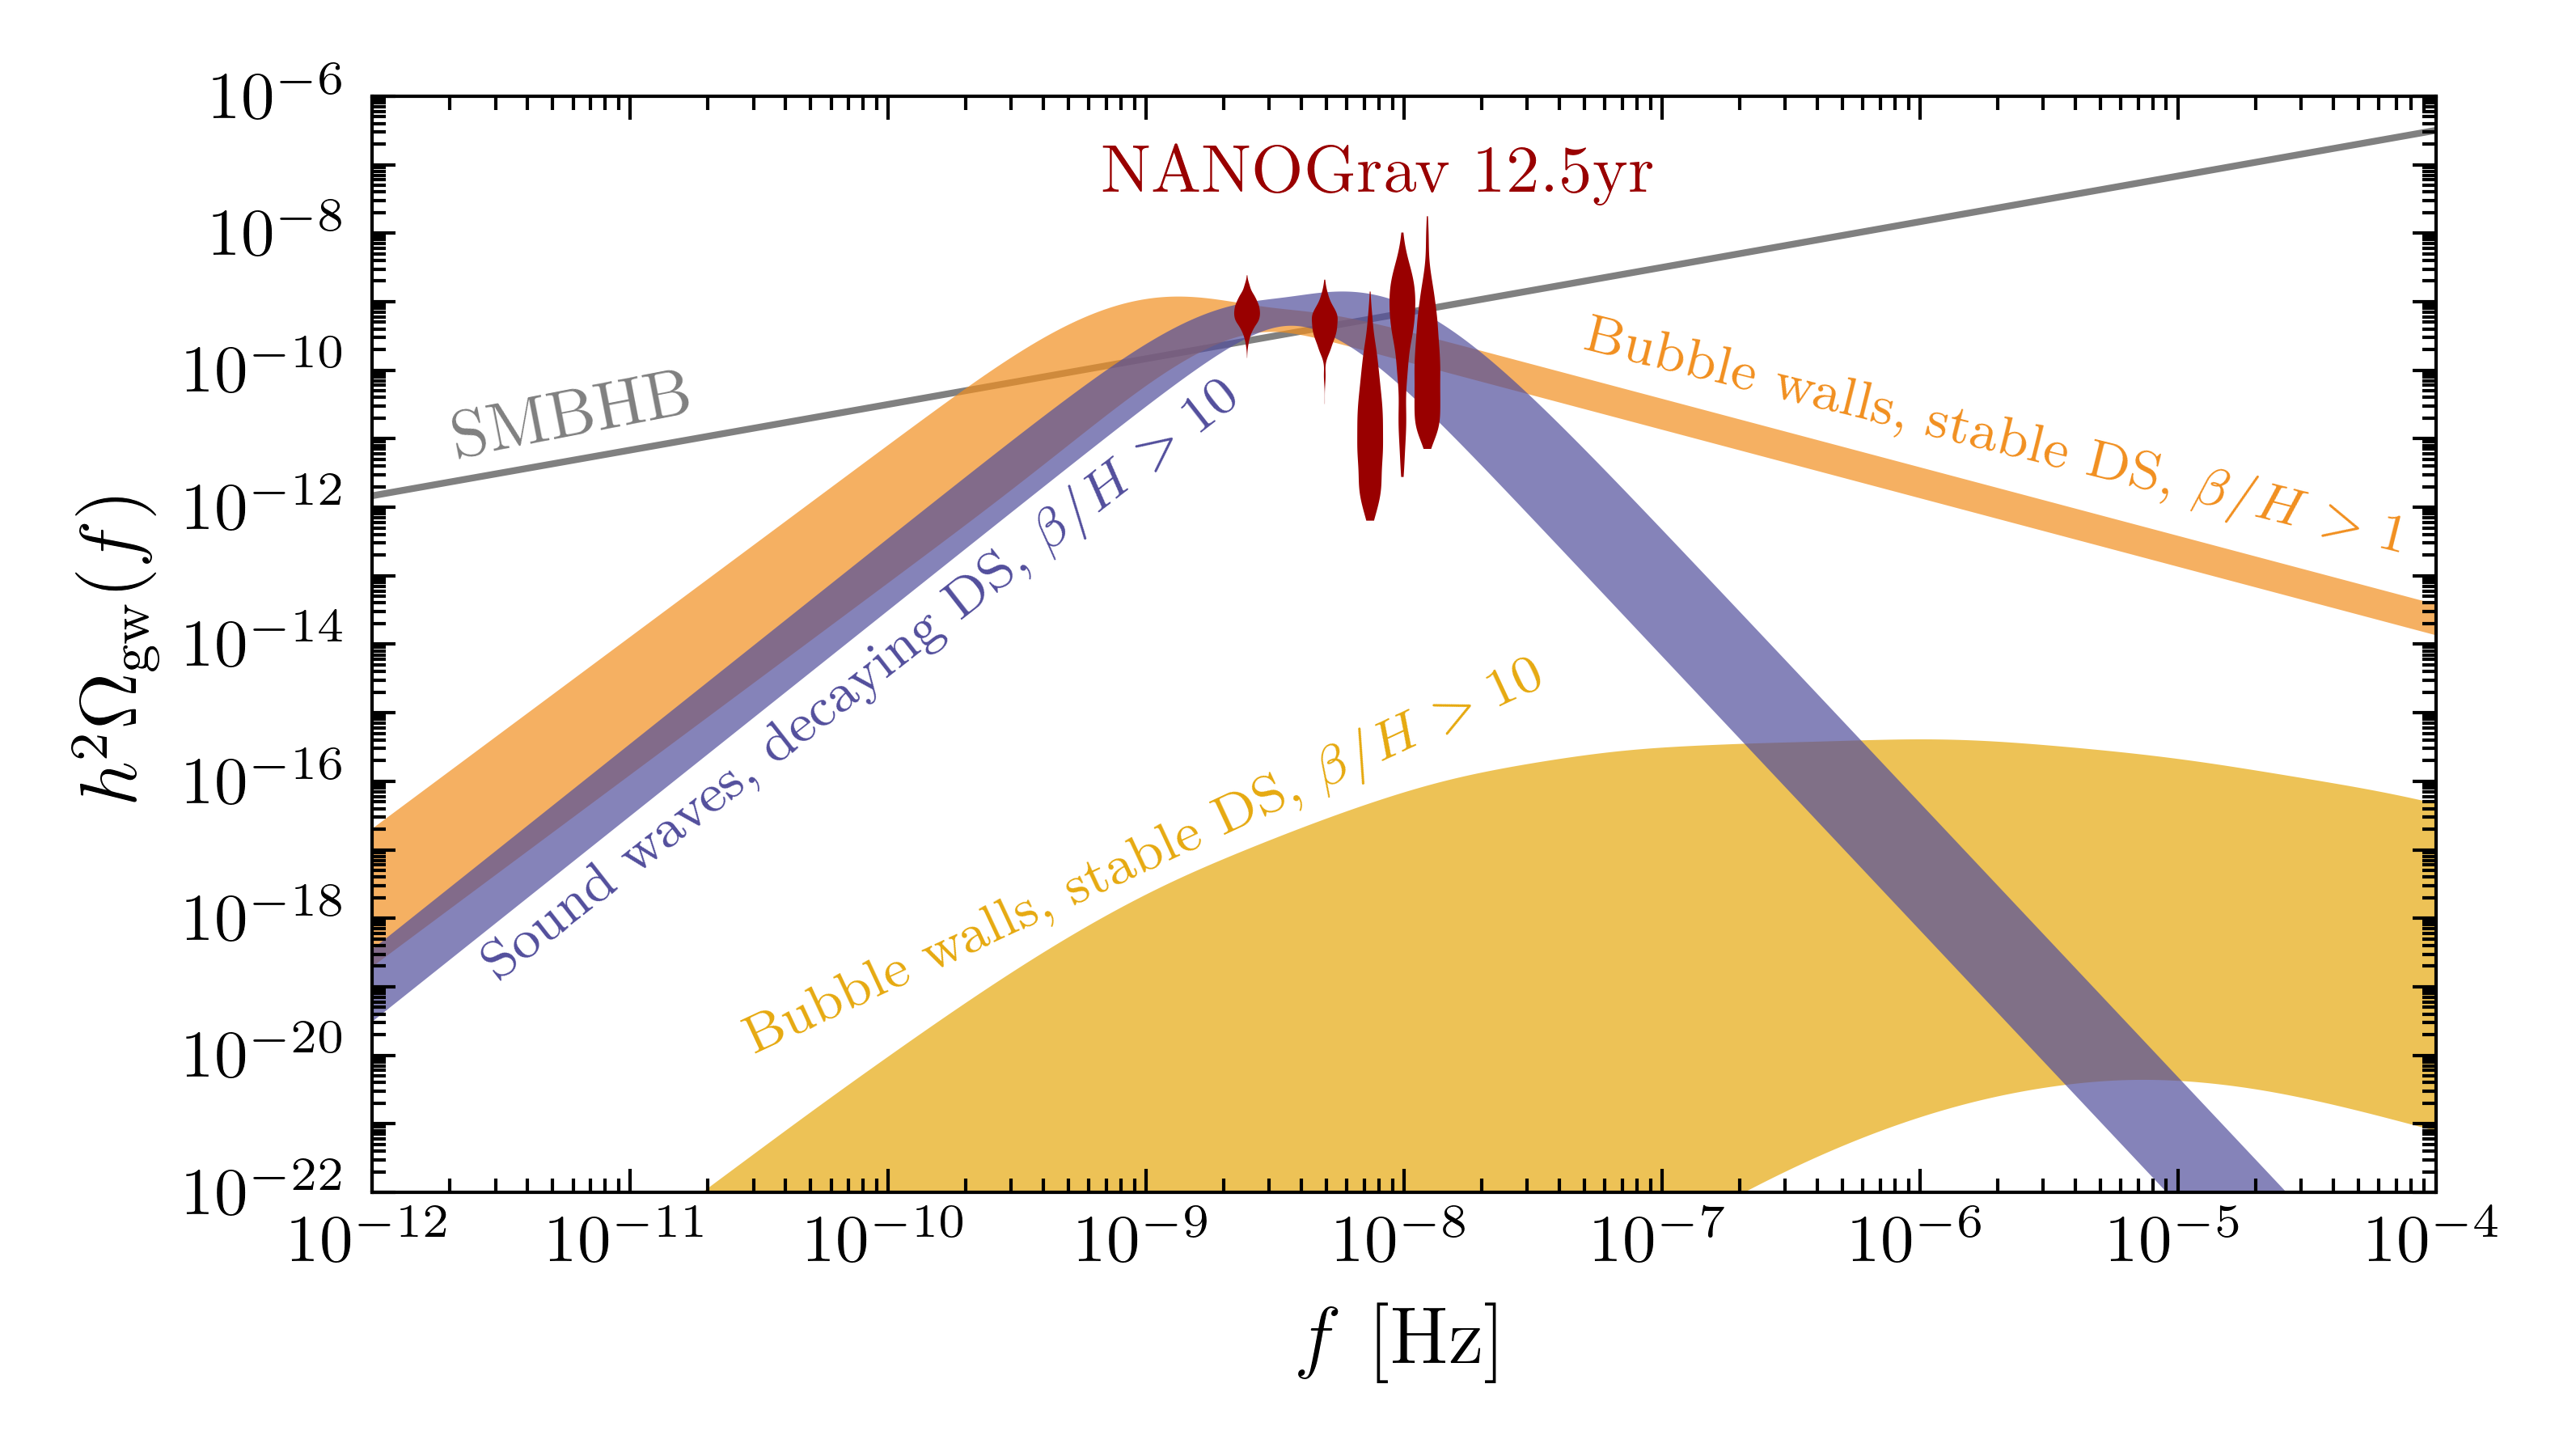
\includegraphics[width = \textwidth]{thesisplots/ptbbn/ptbbn_6}
		\caption{Envelopes of posterior distributions (at $1\sigma$) of \ac{GWB} spectra for parameter scans assuming bubble wall collision spectra from a stable \ac{DSPT} with $\beta/H>1$ (\textcolor{DESYorange}{orange}) and $\beta/H>10$ (\textcolor{DESYgelb}{yellow}), as well as for a decaying \ac{DS} (\textcolor{DESYlila}{violet} spectra). The \ac{GW} from \acp{SMBHB} with $A_\text{SMBHB} = 1.53 \times 10^{-15}$~\cite{NANOGrav:2020bcs} is depicted as a \textcolor{gray}{gray} line for comparison.}
		\label{fig:spec-comparison}
	\end{figure}
	
	\section{Details on the calculation of Bayes factors}
	
	\subsection{The product space method}
	\label{sec:product_space_method}
	The Bayes factor between two models $\mathcal{H}_1$ and $\mathcal{H}_0$ is given by the evidence ratio
	\begin{align}
		\mathcal{B}_{01} = \frac{\mathcal{Z}_1}{\mathcal{Z}_0} \, ,
	\end{align}
	where $\mathcal{Z}_i$ is the evidence of model $i$. The calculation of Bayes factors in this chapter relies on the product space method, which we briefly review here for completeness~\cite{Hee:2015eba,10.2307/1391010, Chamberlin:2014ria, 10.2307/2346151}. In order to compare $\mathcal{H}_0$ and $\mathcal{H}_1$, a hyper-model $\mathcal{H}$ is introduced whose parameter space is given by the Cartesian product $\bm{\theta}_\mathcal{H}$ of the two sub-models' parameters $\bm{\theta}_0$ and $\bm{\theta}_1$ as well as an additional model index $n$ that can formally run from $-0.5$ to $+1.5$. The key idea of this method is that the model index $n$ can be treated as an additional, continuous parameter \graffito{Extending the model parameter space with index $n$} that is sampled over as any other parameter in an \ac{MCMC} chain (while sampling over discrete parameters is technically more challenging). Whenever the hyper-model is evaluated, the underlying algorithm still simply casts the model index to either 0 or 1, corresponding to one of the two sub-models. For a given model index $n$, the hyper-model parameter space is partitioned in an active part, which is used to evaluate the respective likelihood of the sub-model, and an inactive part. The posterior odds ratio $\mathcal{P}_{01}$ is then the relative amount of chain entries in model 1 compared to model 0, from which the Bayes factor $\mathcal{B}_{01}$ between the two models can be deduced.
	
	To demonstrate in some more detail how this procedure can be used to calculate a Bayes factor, consider the posterior probability for the model index $n$
	\begin{align}
		p(n| \text{data}, \mathcal{H}) &= \int \text{d}\bm{\theta}_\mathcal{H} \, p(\bm{\theta}_\mathcal{H}, n  | \text{data}, \mathcal{H}) \nonumber \\ &= \frac{1}{\mathcal{Z}_\mathcal{H}} \int \text{d}\bm{\theta}_\mathcal{H} \, p(\text{data} | \bm{\theta}_\mathcal{H}, n, \mathcal{H}) \, p(\bm{\theta}_\mathcal{H}, n | \mathcal{H}) \, . \label{eq:BF_prob_n}
	\end{align}
	Here the first equality states that the posterior for $n$ can be obtained by marginalizing the posterior for $n$ and $\bm{\theta}_\mathcal{H}$ over the hyper-model parameters. The second equality follows from Bayes' theorem, where $\mathcal{Z}_\mathcal{H}$ is the hyper-model evidence, the first term in the integrand is the likelihood and the second one is the prior for $\bm{\theta}_\mathcal{H}$ and $n$. The hyper-model evidence is unknown and difficult to obtain, but of no further importance, as we are interested in the posterior odds ratio $\mathcal{P}_{01}$ between the two models. For a fixed $n$ we can factorize
	\begin{align}
		p(\bm{\theta}_\mathcal{H}, n | \mathcal{H}) = p(\bm{\theta}_n| \mathcal{H}_n) \, p(\bm{\theta}_{\overline{n}} | \mathcal{H}_{\overline{n}}) \, p(n | \mathcal{H}) \, . \label{eq:BF_prior}
	\end{align}
	This factorization of the prior makes the aforementioned distinction between active (first factor) and inactive (second factor, where $\bar{n}$ refers to all parameters not contained in model $n$) parameters explicit, which are not correlated with each other as \graffito{The posterior odds ratio for model 0 vs.~model 1} the sub-models are distinct. The last factor is an overall, subjective prior for the respective sub-model. The two last factors do not depend on the active parameters $\bm{\theta}_n$. Inserting these expressions into the definition for the posterior odds ratio for the model index $n$, we get 
	\begin{align}
		\mathcal{P}_{01} &\equiv \frac{p(n=1| \text{data}, \mathcal{H})}{p(n=0| \text{data}, \mathcal{H})} \nonumber  \\
		&= \frac{\mathcal{Z}_\mathcal{H}}{\mathcal{Z}_\mathcal{H}} \frac{\int \text{d}\bm{\theta}_\mathcal{H} \, p(\text{data} | \bm{\theta}_\mathcal{H}, n=1, \mathcal{H}) \, p(\bm{\theta}_\mathcal{H}, n=1 | \mathcal{H})}{\int \text{d}\bm{\theta}_\mathcal{H} \, p(\text{data} | \bm{\theta}_\mathcal{H}, n=0, \mathcal{H}) \, p(\bm{\theta}_\mathcal{H}, n=0 | \mathcal{H})} \nonumber  \\
		&= \frac{p(n=1 | \mathcal{H})}{p(n=0 | \mathcal{H})} \, \frac{\int \text{d}\bm{\theta}_1\, p(\text{data} | \bm{\theta}_1, \mathcal{H}_1) \, p(\bm{\theta}_1| \mathcal{H}_1)}{\int \text{d}\bm{\theta}_0 \, p(\text{data} | \bm{\theta}_0, \mathcal{H}_0) \, p(\bm{\theta}_0| \mathcal{H}_0)  } \, \frac{\int \text{d} \bm{\theta}_{\overline{1}} \, p(\bm{\theta}_{\overline{1}} | \mathcal{H}_{\overline{1}})}{\int \text{d} \bm{\theta}_{\overline{0}} \, p(\bm{\theta}_{\overline{0}} | \mathcal{H}_{\overline{0}})}  \nonumber \\
		&= \underbrace{\frac{p(n=1 | \mathcal{H})}{p(n=0 | \mathcal{H})}}_{\equiv \, \Pi_{01}} \quad \times \quad  \underbrace{\frac{\mathcal{Z}_1}{\mathcal{Z}_0}}_{\equiv \, \mathcal{B}_{01}} \, . \label{eq:unit_prior}
	\end{align}
	In the last step we used that the inactive parameters, denoted by a bar, do not contribute to the sub-model evidence $\mathcal{Z}_n$. A marginalization over their priors therefore gives one for both sub-models and the last factor in eq.~(\ref{eq:unit_prior}) equals one. As $\mathcal{P}_{01}$ is just the ratio of the number of chain entries after the burn-in period of sub-model 1 compared to sub-model 0, and the model weight ratio $\Pi_{01}$ can be set as a \graffito{The Bayes factor between models} model prior ratio when starting the \ac{MCMC} chain, the Bayes factor is obtained by multiplying the posterior odds ratio with the inverse model weight ratio,
	\begin{align}
		\mathcal{B}_{01} = \mathcal{P}_{01} \times \Pi_{01}^{-1}\, .\label{eq:BF_BF}
	\end{align}
	
	
	
	\subsection{Uncertainties of the computed Bayes factors}
	
	Our goal is to calculate the Bayes factor as accurately as possible. This can be achieved when the posterior odds ratio $\mathcal{P}_{01}$ is close to one, i.e.~if the hyper-model scan spends about the same amount of time in the two sub-chains. We therefore set the model weight ratio $\Pi_{01}$ to the inverse of the expected Bayes factor and iterate over different \graffito{Most accurate results for $\Pi_{01} \rightarrow 1$} weight ratios until the posterior odds ratio is close to one. In practice, this iterative procedure is still an intricate problem due to long runtimes. When the two models that are compared favor rather different regions of the available pulsar-intrinsic red noise parameter space, jumping from one sub-model to the other is initially unlikely. Hence, the burn-in period is long and uncertainties in the computed Bayes factors increase.
	
	Even though our main aim is to calculate Bayes factors for different \ac{DSPT} scenarios compared to the \ac{NCRN} hypothesis, it is faster and more reliable to first compare a given \ac{DSPT} scenario with the \ac{SMBHB} hypothesis as given in eq.~\eqref{eq:PTA_power_law}. This speeds up the burn-in phase by an $\mathcal{O}(10)$ factor, and results in a more precise computation \graffito{Speeding up the burn-in} of the Bayes factor because the posterior distributions for the pulsar-intrinsic red noise parameters $\{A_a, \gamma_a\}$ are very similar between these two scenarios. As the Bayes factor between \ac{SMBHB} and \ac{NCRN} hypotheses is known, $\log_{10} \mathcal{B}_\text{SMBHB/no-CURN} = 4.5(9)$~\cite{NANOGrav:2020bcs}, and since Bayes factors are multiplicative, $\mathcal{B}_{02} = \mathcal{B}_{01} \times \mathcal{B}_{12}$, we can then simply rescale our results comparing to \ac{SMBHB} to a Bayes factor that compares to the \ac{NCRN} hypothesis. Still, even with an informed choice of $\Pi_{01}$ and using the method outlined above, the chains take several days before the Bayes factor converges. A publicly available implementation of the described pilot run in~ref.~\cite{Chamberlin:2014ria} to speed up the calculation of Bayes factors would therefore be highly appreciated.
	
	Note, however, that the method of first comparing to the \ac{SMBHB} hypothesis does not work if cosmological constraints do not allow a significant \ac{GWB} in a \ac{DSPT} model, like for a stable \ac{DS} with a strong lower bound on $\beta / H$. Here, the \ac{DSPT} models favor similar regions in pulsar-intrinsic red noise parameter space \graffito{Larger uncertainties for weak signals} as in the case of the \ac{NCRN} hypothesis and a direct comparison would be more advantageous. The Bayes factors that we calculate in these cases therefore have larger uncertainties.
	
	Computing Bayes factors inherently involves statistical uncertainties, particularly due to the finite length of the underlying chains. We ensured that this uncertainty is well-managed by calculating the Bayes factor as a function of the number of drawn samples. Using $5 \times 10^6$ samples from the hyper-model (including both sub-models) and \graffito{Statistical uncertainties are under control} conservatively discarding the first $25 \, \%$ due to burn-in, the Bayes factors all converged to a relative uncertainty of a factor of up to $\sim 2$. The convergence rate however depends sensitively on the precise value of the model weights $\Pi_{01}$ as mentioned above. We therefore made sure that the number of samples of both models differed by no more than $\mathcal{O}(10 \, \%)$, which requires to (iteratively) find the model weights $\Pi_{01}$ up to one decimal place.
	
	The continuous lines in fig.~\ref{fig:BFs}, depicting the Bayes factor expected prior dependencies, are further prone to uncertainties due to the reduction of points after adapting the prior, cf.~appendix~\ref{sec:priorchoice}. This is particularly relevant when this reduction is large, i.e.~when the Bayes factor is reduced by a significant amount, e.g.~for a \ac{GWB} from bubble wall collisions and a large lower boundary for $\beta / H$. Taken together, these uncertainties are the reason for the differences compared to the individually calculated Bayes factors for a given prior choice (solid dots).
	
	
	\subsection{Relating Bayes factors to $p$-values and $Z$-scores}
	\label{sec:z-scores}
	Bayes factors can be expressed in terms of a ``$Z$-score'' to describe the (im)probability of the null hypothesis~\cite{Athron:2020maw,Fowlie:2019ydo}, more commonly known as the ``number of sigmas'' with which some measured quantity deviates from \graffito{``How many $\sigma$ is $\mathcal{B} = 10^3$?''} its expectation value. The probability of the null hypothesis can be interpreted as $p(0|\text{data}) = 1 - p(1|\text{data})$ in a frequentist's manner, if one asserts that there is no other possible model to explain the data. If one further interprets the posterior odds ratio to be the ratio of these probabilities $\mathcal{P}_{01} = p(1|\text{data}) / p(0|\text{data})$, one obtains $p(0|\text{data}) = 1/(1 + \mathcal{P}_{01})$. This can be interpreted as a $p$-value, i.e.~the probability to measure data as extreme as the one observed if the null hypothesis were indeed correct. Assuming equal prior probabilities for the two models under comparison, i.e.~$\Pi_{01} = 1$, the $p$-value reads $p = 1/(1 + \mathcal{B}_{01})$, which formally corresponds to $\mathcal{P}_{01}=\mathcal{B}_{01}$. We convert the obtained $p$-value to a $Z$-score using a one-tailed Gaussian,
	\begin{align}
		Z = \Phi^{-1}(1 - p) = \Phi^{-1} \ba{\frac{1}{1 + {1}/{\mathcal{B}_{01}}}} \,, \label{eq:z-score}
	\end{align}
	where $\Phi^{-1}$ is the inverse of the cumulative density function of the standard normal distribution with zero  mean and unit standard deviation. 
	
	For Bayes factors $\mathcal{B}_{01}$ below 1 we replace $\mathcal{B}_{01}$ by its inverse, in order to express the tension between data sets if the null hypothesis is a better explanation for the observed data than a given, more complicated model. In that case the interpretation of $Z$ is related to the probability of obtaining a signal as low as 
	observed if the signal model were indeed correct.
	
	
	\subsection{Influence of the prior choice on the Bayes factor}
	\label{sec:priorchoice}
	
	We now want to investigate the effect of a change in prior $\pi(\bm{\theta}) \rightarrow \tilde{\pi}(\bm{\theta})$ on the Bayes factor $\mathcal{B}_{01} \rightarrow \mathcal{B}_{0{\tilde{1}}}$ (in this section, we denote for \graffito{The Bayes factor correction $R$} simplicity the model parameters of model 1 by $\bm{\theta}$). Keeping the likelihood and its normalization as well as the number of model parameters unchanged, the Bayes factors differs by a factor
	\begin{align}
		R \equiv \frac{\mathcal{B}_{0{\tilde{1}}}}{\mathcal{B}_{01}} =  \frac{\mathcal{Z}_{\tilde{1}}}{\mathcal{Z}_0}  \cdot \frac{\mathcal{Z}_0}{\mathcal{Z}_1} =  \frac{\int \diff\bm{\theta} \, \mathcal{L}(\bm{\theta}) \,  \tilde{\pi}(\bm{\theta}) }{\int \diff\bm{\theta} \, \mathcal{L}(\bm{\theta}) \,  \pi(\bm{\theta}) } \, .
	\end{align}
	Flat, proper priors (as assumed throughout this thesis) take a very simple form satisfying
	\begin{align}
		1 = \int \diff \bm{\theta} \, \pi(\bm{\theta}) = \frac{1}{V_\pi} \int_{V_\pi} \diff \bm{\theta} && \text{and} && 1 = \int \diff \bm{\theta} \, \tilde{\pi} (\bm{\theta}) = \frac{1}{V_{\tilde{\pi}} }   \int_{V_{\tilde{\pi}}} \diff \bm{\theta} \, ,
	\end{align}
	where $V_\pi$ is the prior volume. In this case, the Bayes factor ratio simplifies to
	\begin{align}
		R  = \frac{V_\pi}{V_{\tilde{\pi}}} \, \frac{\int_{V_{\tilde{\pi}}} \diff \bm{\theta} \,  \mathcal{L}(\bm{\theta})}{\int_{V_\pi} \diff \bm{\theta} \, \mathcal{L}(\bm{\theta})} \, . \label{eq:BF_prior_dependence1}
	\end{align}
	The effect of changing the range of a flat prior can thus be understood intuitively: Increasing the prior into a region where the likelihood is negligible comes with the cost of increased prior volume, while the posterior integral is largely unaffected. If the likelihood were instead globally flat, an increase in prior volume would have no effect on the Bayes factor, \graffito{$R$ compares the posterior-to-prior volume ratio change for two prior choices} as the increase in the posterior would just be compensated by the increased prior volume. This simply reflects the well-known feature of Bayesian statistics to disfavor unnecessary model complexity. In other words, the cost of introducing a new parameter depends on the coverage of the prior volume with the posterior. If the posterior of this parameter is flat, it can be introduced without changing the Bayes factor. If it however needs to be fine-tuned to fit the data, i.e.~if its posterior is only a thin peak, the coverage of the prior volume is low, reducing the Bayes factor.
	
	The above considerations allow us to reduce the prior ranges after having computed a Bayes factor for some prior ranges that we initially set too wide, without \graffito{For flat priors, $R$ can be computed easily} the need to start a new \ac{MCMC} chain. This is possible as the chain entries are distributed following the model likelihood $\mathcal{L}(\bm{\theta})$ (being proportional to the posterior for a flat prior). The ratio of integrals in eq.~\eqref{eq:BF_prior_dependence1} thus reduces to a ratio of chain entries,
	thereby changing the Bayes factor as 
	\begin{align}
		R  \rightarrow \frac{V_\pi}{V_{\tilde{\pi}}} \,  \frac{N_{\tilde{\pi}}} {N_\pi} \, ,
	\end{align}
	where $N_{\tilde{\pi}}$ and $N_\pi$ are the number of chain entries enclosed within the prior volumes $V_{\tilde{\pi}}$ and $V_\pi$ respectively. Note that this ``a-posteriori'' change of the priors is not more than a tool to quickly \textit{estimate} the effect of slightly reducing of the prior volume. As soon as one cuts away a region of parameter space that was initially well-covered by the prior, the above approximation comes with an increased statistical error due to a potentially low number of samples $N_{\tilde{\pi}}$. This can for instance be seen by looking at the red line in fig.~\ref{fig:BFs}. It should also be noted that the uncertainty of this approximation does not scale with $1/\sqrt{N_{\tilde{\pi}}}$ due to the immanent properties of importance sampling which were required to evaluate the ratio of posterior integrals in the first place. A considerable reduction of the prior therefore comes with a significant error, in practice still requiring the computation of a full new \ac{MCMC} chain with the updated prior ranges.
	
	The effect of changing the prior range is also illustrated in fig.~\ref{fig:priordependence}, where we show the Bayes factor ratio for \acp{SMBHB} with different choices of lower and upper prior boundaries on the amplitude $A_\text{SMBHB}$. As the posterior for the amplitude peaks between $10^{-15}$ and $10^{-14.5}$, the lower boundary of $10^{-18}$ on the \graffito{Evidence for \ac{SMBHB} can grow by a factor four} log prior could be doubted to be a good choice, cf.~ref.~\cite{Casey-Clyde:2021xro}. If one instead chose the lower boundary to lie at $10^{-15}$, a factor four increase in the \ac{SMBHB}'s model evidence would be expected. Only lowering the upper prior boundary from $10^{-14}$ down to $10^{-14.5}$, on the other hand, would barely change the Bayes factor as this cuts away  only a tiny amount of the prior parameter space that is favored by the posterior distribution.
	\begin{figure}[t]
		\centering
		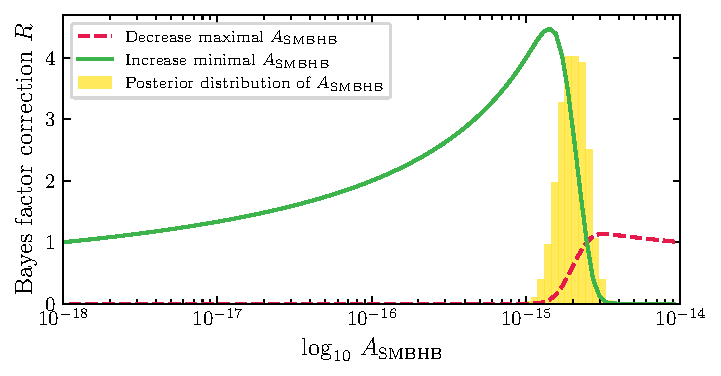
\includegraphics[width=\linewidth]{thesisplots/ptbbn/ptbbn_7}
		\caption{Bayes factor dependence on the $A_\text{SMBHB}$ prior range for a SMBHB signal when increasing the lower boundary (\textcolor{PlotGreen}{green} line) and lowering the upper boundary (\textcolor{PlotRed}{red} line). The posterior distribution of the \ac{SMBHB} \ac{GWB} spectral amplitude $A_\text{SMBHB}$ is shown in \textcolor{PlotYellow}{yellow}.}
		\label{fig:priordependence}
	\end{figure}
	
	
	\subsection{Influence of priors on the credibility of a DSPT}
	\label{sec:priorsDSPT}
	
	Interpreting the results of Bayesian statistics can be challenging given that posteriors and therefore also model evidences and Bayes factors are prior-dependent (even though this of course makes sense in the Bayesian framework, where prior beliefs should be updated when taking into account measured data). Not the least to assess the robustness of our main findings we therefore want to investigate the influence of prior choices on the Bayes factors. Concretely, let us get back to the main question brought up in section \ref{sec:results_comp}: does the discrepancy between the Bayes factors for a decaying \ac{DSPT} and the \ac{SMBHB} interpretation, cf.~fig.~\ref{fig:BFs}, have anything to do with the goodness-of-fit of the two explanations -- or is it completely dominated by prior-volume effects?
	
	In order to answer this question, we used a twofold approach: First we identified the region of parameter space that results in the highest posterior probabilities. Then we started two chains, one where all priors were constrained to only cover the best-fit regions\footnote{We chose the following log prior ranges in this case: $\alpha \in \bb{0.02, 0.04}$, $\beta/H \in \bb{1, 3}$, $T_\perc / \text{MeV} \in \bb{10, 100}$, $\xi_\perc \in \bb{0.01, 0.1}$, $\tau_\phi / \text{s} \in \bb{0.01, 0.1}$.} and a second one in which we fixed all model parameters to their best-fit values\footnote{Specifically, we chose $\beta/H = 10^{0.3} = 2$, $T_\perc = 10^{-1.6} \, \text{GeV} = 25 \, \text{MeV}$, $\xi_\perc = 0.01$, $\tau = 10 \, \text{ms}$. These values were chosen somewhat arbitrarily and are not the result of a precise maximization of the posterior probability. It is thus conceivable that a slightly better fit to the common red spectrum could be obtained by fine-tuning the parameter points.} except \graffito{An equal footing for model priors}  for $\alpha$, for which we adopted a log prior in the range $\bb{10^{-3}, 10^{1}}$. In doing so the prior in the second approach spans over four orders of magnitude, just as the prior for $A_\text{SMBHB} \in \bb{10^{-18}, 10^{-14}}$, which allows for a comparison of the two models on a similar footing.
	
	In the first analysis we obtained a Bayes factor of $\sim5$ between the decaying \ac{DSPT} and \ac{SMBHB} interpretation in \textit{favor} of the \ac{DSPT} hypothesis. The second analysis found a Bayes factor of $\sim1.4$, again in (very slight) favor of the decaying \ac{DSPT} interpretation. We checked explicitly that this matches the expected \graffito{\acp{DSPT} can fit the data slightly better than \acp{SMBHB}} Bayes factors from an ``a-posteriori'' prior change as described in appendix~\ref{sec:priorchoice}. Both Bayes factors are also consistent with each other, since the one of the second analysis could be enhanced by a factor of $4$ if one decreased the prior range to one decade, $\alpha \in \bb{10^{-2}, 10^{-1}}$, confirming the $\sim5$ Bayes factor of the first analysis. To make this a fair comparison it should however be noted that also the evidence of the \ac{SMBHB} hypothesis can be boosted by a relative factor of $4$ by decreasing the prior range of $A$ from $\bb{10^{-18}, 10^{-14}}$ to $\bb{10^{-15}, 10^{-14}}$, cf.~fig.~\ref{fig:priordependence} in appendix~\ref{sec:priorchoice}.
	
	We therefore conclude that a \ac{GWB} with a broken power-law spectrum with fixed slopes $\Omega_\text{sw}(f) \propto f^3$ and 
	$\Omega_\text{sw}(f) \propto f^{-4}$ for low and high \graffito{Prior choices result in the difference between $\mathcal{B} = 10^{4.5}$ and $\mathcal{B} = \mathcal{O}(200)$}  frequencies respectively, can in principle fit the common red spectrum slightly better than a featureless single power-law with spectral index $\gamma_\text{SMBHB} = 13/3$. As discussed further in section \ref{sec:results_comp}, the origin of the discrepancy between the highest Bayes factors depicted in fig.~\ref{fig:BFs} and the reference value of $\sim10^{4.5}$ is thus indeed due to prior volume effects. 
	
	\clearpage
	
	\subsection{Priors for the Bayesian model comparison}
	\label{sec:priors}
	
	\mbox{}
	\vspace{12em}
	\begin{center}
		\begin{sideways}
			\begin{minipage}{\linewidth}
				\scriptsize
				\begin{tabular}{| l | c| c| c| c|c|c|c|c|}
					\hline
					\multicolumn{1}{|c|}{ \textbf{Parameter}} & \multicolumn{3}{|c|}{~~~~~\textbf{Description}~~~~~} & \multicolumn{2}{|c|}{~~~~\textbf{Prior}~~~~} & \multicolumn{3}{|c|}{~~\textbf{Comments}~~} \\
					\hline\hline
					\multicolumn{9}{|c|}{\textbf{PSR-intrinsic red noise}}\\
					\hline\hline
					$A_{a}$& \multicolumn{3}{|c|}{Red noise power-law amplitude} & \multicolumn{2}{|c|}{log-Uniform $[-20,-11]$} & \multicolumn{3}{|c|}{one parameter per pulsar} \\
					$\gamma_{a}$& \multicolumn{3}{|c|}{Red noise power-law spectral index} & \multicolumn{2}{|c|}{Uniform $[0,7]$} & \multicolumn{3}{|c|}{one parameter per pulsar} \\
					\hline\hline
					\multicolumn{9}{|c|}{\textbf{Supermassive Black Hole Binaries (SMBHBs)}}\\
					\hline\hline
					$A_{\text{SMBHB}}$& \multicolumn{3}{|c|}{Red noise power-law amplitude} & \multicolumn{2}{|c|}{log-Uniform $[-18,-14]$} & \multicolumn{3}{|c|}{one parameter for PTA} \\
					\hline\hline
					\multicolumn{9}{|c|}{\textbf{Stable dark sector phase transition, sound wave or bubble wall collision spectrum}}\\
					\hline\hline
					$\alpha$& \multicolumn{3}{|c|}{Phase transition strength} & \multicolumn{2}{|c|}{log-Uniform $[-5, 1]$} & \multicolumn{3}{|c|}{one parameter for PTA} \\
					$\beta/H$& \multicolumn{3}{|c|}{Inverse timescale} & \multicolumn{2}{|c|}{
						\begin{tabular}{@{}c@{}}log-Uniform $[0, 3]$, $[\log_{10} 3 , 3]$, \\ $[\log_{10} 5 , 3]$, $[\log_{10} 7, 3]$, $[1, 3]$\end{tabular}			
					} & \multicolumn{3}{|c|}{one parameter for PTA} \\
					$T_\perc / \text{GeV}$& \multicolumn{3}{|c|}{SM temperature at percolation} & \multicolumn{2}{|c|}{log-Uniform $[-4, 1]$} & \multicolumn{3}{|c|}{one parameter for PTA}\\
					$\xi_\perc$& \multicolumn{3}{|c|}{DS temperature ratio at percolation} & \multicolumn{2}{|c|}{log-Uniform $[-2, 1]$} & \multicolumn{3}{|c|}{one parameter for PTA}\\
					$g_\text{DS}$& \multicolumn{3}{|c|}{DS degrees of freedom} & \multicolumn{2}{|c|}{Constant $1$} & \multicolumn{3}{|c|}{one parameter for PTA}\\
					$D$& \multicolumn{3}{|c|}{Dilution factor} & \multicolumn{2}{|c|}{Constant $1$} & \multicolumn{3}{|c|}{one parameter for PTA}\\
					\hline\hline
					\multicolumn{9}{|c|}{\textbf{Decaying dark sector phase transition, sound wave spectrum}}\\
					\hline\hline
					$\alpha$& \multicolumn{3}{|c|}{Phase transition strength} & \multicolumn{2}{|c|}{log-Uniform $[-3, 1]$} & \multicolumn{3}{|c|}{one parameter for PTA} \\
					$\beta/H$& \multicolumn{3}{|c|}{Inverse timescale} & \multicolumn{2}{|c|}{
						\begin{tabular}{@{}c@{}}log-Uniform $[0, 3]$, $[\log_{10} 3 , 3]$, \\ $[\log_{10} 5 , 3]$, $[\log_{10} 7, 3]$, $[1, 3]$\end{tabular}			
					} & \multicolumn{3}{|c|}{one parameter for PTA} \\
					$T_\perc / \text{GeV}$& \multicolumn{3}{|c|}{SM temperature at percolation} & \multicolumn{2}{|c|}{log-Uniform $[-4, 0]$} & \multicolumn{3}{|c|}{one parameter for PTA}\\
					$\xi_\perc$& \multicolumn{3}{|c|}{DS temperature ratio at percolation} & \multicolumn{2}{|c|}{log-Uniform $[-3, 1]$} & \multicolumn{3}{|c|}{one parameter for PTA}\\
					$\tau_\phi / \text{s}$& \multicolumn{3}{|c|}{Dark Higgs lifetime} & \multicolumn{2}{|c|}{log-Uniform $[-6,2]$} & \multicolumn{3}{|c|}{one parameter for PTA}\\
					$g_\text{DS}$& \multicolumn{3}{|c|}{DS degrees of freedom} & \multicolumn{2}{|c|}{Constant $1$} & \multicolumn{3}{|c|}{one parameter for PTA}\\
					$D$& \multicolumn{3}{|c|}{Dilution factor} & \multicolumn{2}{|c|}{Constant $1$} & \multicolumn{3}{|c|}{one parameter for PTA}\\
					$m_\phi / \, \text{MeV}$& \multicolumn{3}{|c|}{Dark Higgs mass} & \multicolumn{2}{|c|}{Constant $5$} & \multicolumn{3}{|c|}{one parameter for PTA}\\		
					\hline
				\end{tabular}
			\end{minipage}
		\end{sideways}
		\captionof{table}{Table showing the model parameters together with their respective prior ranges.}
		\label{tab:priors}
	\end{center}

\unappendix
